\documentclass[11pt]{article}
\usepackage[margin=1in]{geometry}
\usepackage{authblk}
\usepackage{amsmath,amssymb}
\usepackage{graphicx}
\usepackage{caption}
\usepackage{subcaption}
\usepackage{placeins}
\usepackage[numbers,sort&compress]{natbib}
\usepackage{hyperref}
\hypersetup{colorlinks=true,linkcolor=black,citecolor=black,urlcolor=black}

\title{Phase Transitions in Collective Emotion: A Theoretical Framework Motivated by Media Dynamics During the COVID-19 Pandemic}
\author[1]{Author A (TBD)}
\affil[1]{Affiliation TBD}
\date{}

\begin{document}
\maketitle

\begin{abstract}
Information ecosystems can abruptly shift into polarized emotional states, yet prediction remains difficult because heterogeneous media feedback and individual psychological thresholds interact nonlinearly. We introduce a mixed-feedback model in which mainstream media provides stabilizing negative feedback and ``We-media'' provides amplifying positive feedback. Their competition is controlled by a single removal ratio that yields an analytic critical point $r_c$ and a Ginzburg-Landau potential that predicts pitchfork bifurcation and critical slowing down. Agent-based network simulations reproduce these theoretical signatures and map how thresholds, information density, media ecology, and local coupling shift the effective transition point. We then test empirical implications on large-scale Weibo data by operationalizing polarization $Q$, activity $a$, and a media-composition proxy $r_{\text{proxy}}$. The activity-to-jump link (H1) is supported in the pooled dataset, while the media-volatility prediction (H2) is supported in batch3 but weakens after controlling for sampling density, indicating an important confound. Early-warning signals based on critical slowing down (H4) are inconclusive under current data continuity and event sparsity, providing a boundary on empirical observability of the theoretical signature.
\end{abstract}

\noindent\textbf{Keywords:} phase transitions, collective emotion, mixed-feedback, emotional bubbles, critical slowing down, COVID-19

\section{Introduction}
Understanding abrupt, nonlinear transitions in collective behavior---from opinion polarization and market crashes to social unrest---remains a central challenge in computational social science. Many models capture gradual change, but they often struggle to explain system-wide shifts that emerge from nonlinear feedback and networked interactions \citep{Centola2010,Watts2002,Becker2017,Hasell2021,Chong2018,Lerman2024,Helfmann2023,Giacomo2025,Piao2023}. These dynamics are particularly salient in online information ecosystems, where algorithmic amplification and adaptive exposure can push public sentiment toward tipping points.

The COVID-19 pandemic provided a global-scale context in which public emotion evolved alongside an ``infodemic'' of heterogeneous risk information \citep{Green2020,Bavel2020,Wang2022,Aslam2020,Chou2020,Liu2024}. A recurring empirical observation is that different media sources can play opposing roles: mainstream media often moderates sentiment, while independent social accounts amplify high-arousal narratives. This pattern echoes risk amplification frameworks \citep{Kasperson1988} and related studies on moral outrage and emotional contagion \citep{Goldenberg2021,Brady2023,Crockett2017,Kramer2014,Fan2014}, yet it is not captured by single-channel amplification models. We refer to the resulting abrupt regime shifts as emotional bubbles, by analogy to financial bubbles that appear stable until a critical threshold is crossed.

To address this puzzle, we develop a parsimonious mixed-feedback model that treats mainstream media as stabilizing negative feedback and ``We-media'' as amplifying positive feedback. The balance between them is controlled by a single parameter $r$, allowing a controlled sweep from consensus to polarized regimes. We combine mean-field analysis with agent-based simulations and then link theoretical predictions to empirical proxies in Weibo data. The goal is not to fit a crisis-specific model, but to establish a mechanism-based, testable framework for collective emotion dynamics under competing feedback.

\section{Materials and Methods}
\subsection{Mixed-feedback model framework}
We consider a population of $N$ individuals with three arousal states: high ($H$), medium ($M$), and low ($L$). Let $(\rho_H,\rho_M,\rho_L)$ denote the population fractions with $\rho_H+\rho_M+\rho_L=1$. We introduce two orthogonal macroscopic variables: the polarization direction
\begin{equation}
q(t)=\rho_H(t)-\rho_L(t),
\label{eq:q}
\end{equation}
and the system activity
\begin{equation}
a(t)=\rho_H(t)+\rho_L(t)=1-\rho_M(t).
\label{eq:a}
\end{equation}
These order parameters decouple symmetry breaking from the depletion of the moderate buffer, with $\rho_H=(a+q)/2$ and $\rho_L=(a-q)/2$.

At each update, an individual samples $k$ risk signals from the environment, each labeled ``risk'' with probability $p_i$. Let $S\sim\text{Binomial}(k,p_i)$ denote the number of risk signals and $\hat{p}=S/k$ the perceived risk fraction. Individuals transition to $H$ if $\hat{p}\ge\phi$, to $L$ if $\hat{p}\le\theta$, and otherwise remain in $M$, where $\theta<\phi$ define low and high arousal thresholds.

The information environment is modeled as a competition between mainstream media (negative feedback) and We-media (positive feedback). The mainstream signal is
\begin{equation}
p^{\text{main}}(q)=\frac{1-q}{2},
\label{eq:pmain}
\end{equation}
which counteracts the current polarization. For We-media we use two regimes. In the symmetric validation regime, used for analytical verification, we set
\begin{equation}
p^{\text{we}}(q)=\frac{1}{2}+\frac{q}{2},
\label{eq:pwe_sym}
\end{equation}
which enforces $q\to -q$ symmetry. In the asymmetric, realistic regime we allow activity coupling via
\begin{equation}
p^{\text{we}}(q,a)=\rho_H=\frac{a+q}{2}.
\label{eq:pwe_asym}
\end{equation}
The overall environmental risk is the weighted average
\begin{equation}
p_{\text{env}}(q,a;r)=\frac{(1-r)n_m p^{\text{main}} + r n_w p^{\text{we}}}{(1-r)n_m + r n_w}, \qquad r\in[0,1],
\label{eq:penv}
\end{equation}
where $n_m$ and $n_w$ are the baseline strengths of mainstream and We-media sources, and $r$ is the mainstream removal ratio.

\subsection{Mean-field analysis and critical point}
Under the symmetric regime, $q=0$ is a fixed point with $p_{\text{env}}=1/2$. Linearizing the mean-field dynamics around $q=0$ yields
\begin{equation}
\frac{dq}{dt}=-q+\mathcal{S}(p),
\label{eq:q_dynamics}
\end{equation}
where $\mathcal{S}(p)$ is the collective response. We define the psychological sensitivity
\begin{equation}
\chi=\left.\frac{d\mathcal{S}}{dp}\right|_{p=1/2},
\label{eq:chi}
\end{equation}
and the feedback gradient $\Gamma=\left.\partial p_{\text{env}}/\partial q\right|_{q=0}$. The stability condition $\chi\Gamma=1$ gives the analytic critical point
\begin{equation}
r_c=\frac{n_m(\chi+2)}{n_m(\chi+2)+n_w(\chi-2)}.
\label{eq:rc}
\end{equation}
Near $r\approx r_c$, the order parameter obeys a Ginzburg-Landau form,
\begin{equation}
\frac{dq}{dt}=-\frac{\partial V_{\text{eff}}(q)}{\partial q}+\eta(t),\qquad V_{\text{eff}}(q)=\frac{1}{2}\alpha q^2+\frac{u}{4}q^4,
\label{eq:gl}
\end{equation}
with $\alpha\propto(r_c-r)$ and $u>0$, predicting a pitchfork bifurcation and critical slowing down, $\tau\sim 1/|r_c-r|$.

\subsection{Agent-based network simulations}
We simulate microscopic dynamics on ER and BA networks with size $N$ and average degree $\langle k\rangle$. Updates are asynchronous: each step updates a fraction of nodes, and we report time in both steps and sweeps. Local coupling $\beta$ mixes the global signal $p_{\text{env}}$ with neighbor information, allowing us to quantify how topology and local reinforcement shift the effective transition. For symmetric systems we measure $|Q|$ or aligned signed $Q$ to avoid cancellation from random branch selection, and we estimate finite-size transition points using Binder cumulant crossings,
\begin{equation}
U_4(r;N)=1-\frac{\langle Q^4\rangle}{3\langle Q^2\rangle^2}.
\label{eq:binder}
\end{equation}

\subsection{Empirical data and operational proxies}
Empirical validation uses Weibo data spanning January 2020 to December 2023, including mainstream media, We-media, and public posts. Texts are labeled for emotional arousal and risk content via a DistilBERT-based classifier \citep{Sanh2020}. We construct time series for polarization $Q= X_H-X_L$ and activity $a=X_H+X_L$ from aggregated arousal fractions. Media composition is proxied by
\begin{equation}
r_{\text{proxy}}=\frac{n_{\text{wemedia}}}{n_{\text{wemedia}}+n_{\text{mainstream}}+n_{\text{government}}},
\label{eq:rproxy}
\end{equation}
with government accounts included in the official-narrative denominator. We aggregate time series at 4H resolution and compute segment-level statistics. H1 links activity to jump intensity using the segment-level 95th percentile of $|d|Q|/dt|$; H2 links $r_{\text{proxy}}$ to volatility defined as $\text{std}(Q)$ within segments; H4 probes critical slowing down using rolling $AC1(|Q|)$ and $\mathrm{Var}(|Q|)$ before jump events with block-aware placebo tests.

\section{Results}
\subsection{Theoretical bifurcation and critical point}
In the symmetric validation regime, the model exhibits a pitchfork bifurcation as the control parameter $r$ crosses the analytic threshold $r_c$. For the baseline configuration $n_m=10$, $n_w=5$, $\phi=0.54$, $\theta=0.46$, and $k=50$, the theory predicts $r_c\approx 0.753$. The bifurcation structure is captured by the order parameter $q$ and is directly explained by the effective potential $V_{\text{eff}}(q)$, which transitions from a single well to a double well as $r$ increases (Fig.~\ref{fig:theory}). This establishes a mechanistic interpretation of emotional bubbles: as negative feedback is weakened, the system becomes bistable and small perturbations select one polarized branch.

\begin{figure}[t]
  \centering
  \begin{subfigure}[b]{0.48\linewidth}
    \centering
    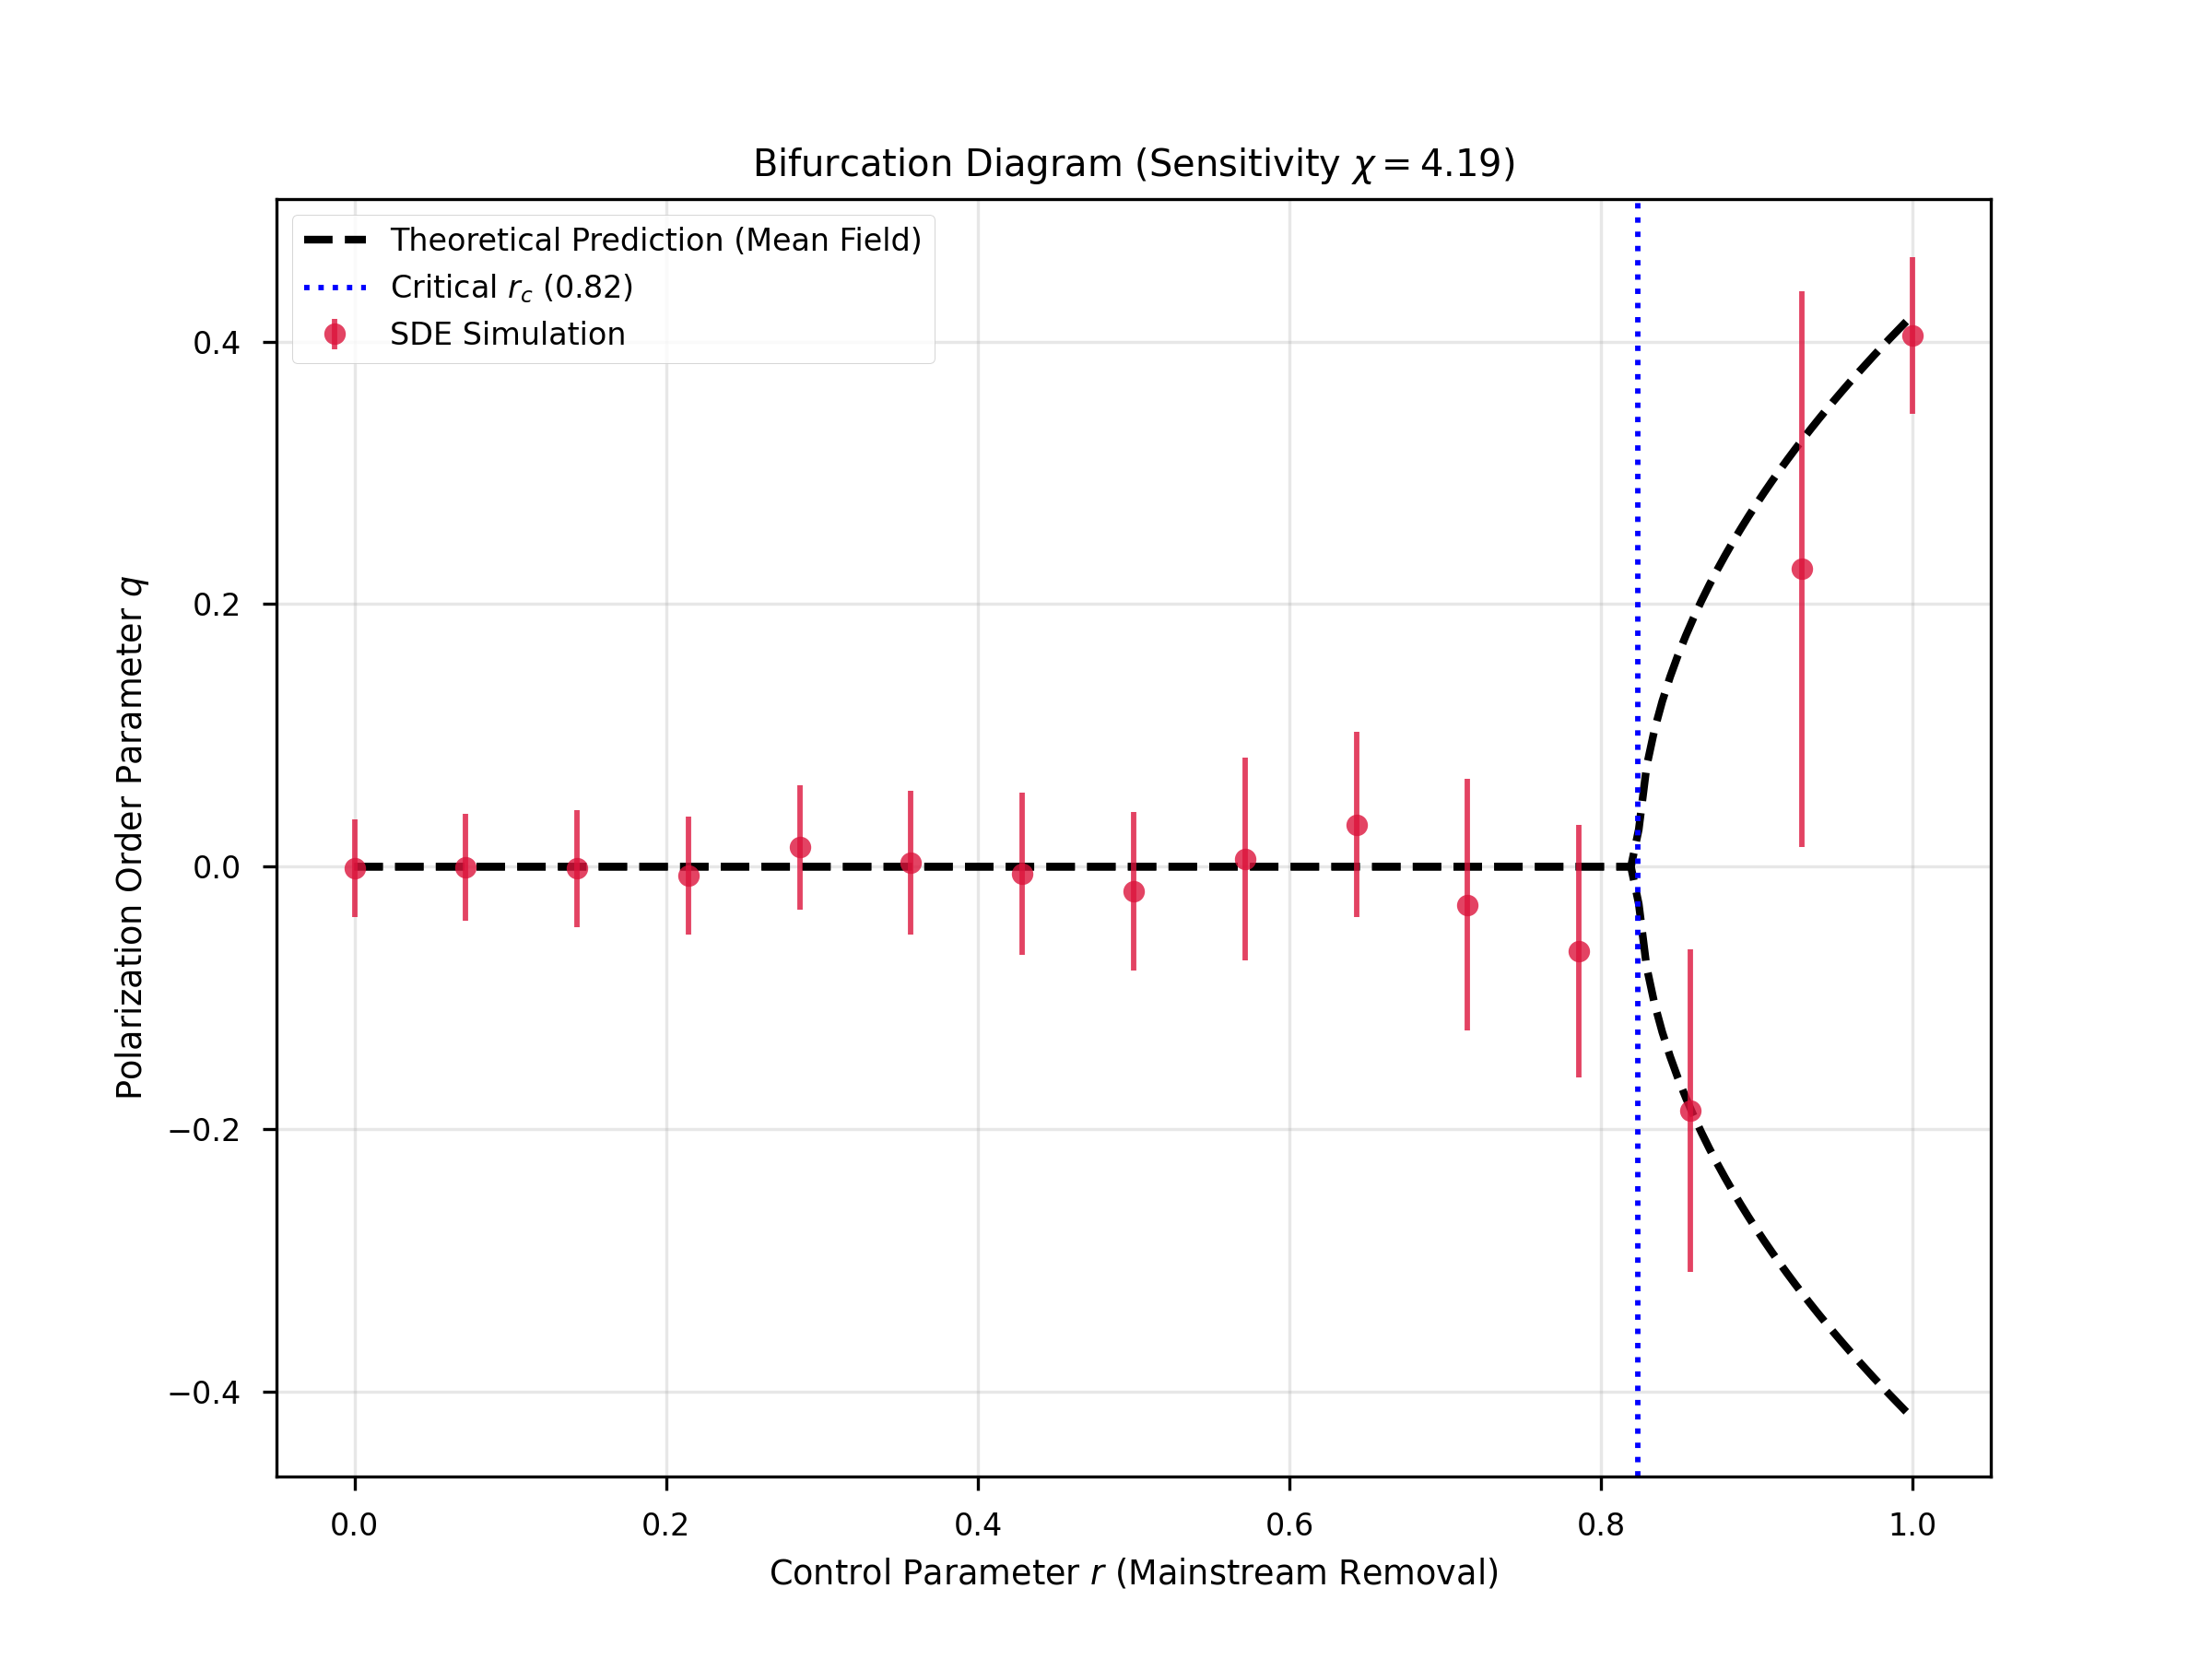
\includegraphics[width=\linewidth]{figures/fig1a_bifurcation.png}
    \caption{}
  \end{subfigure}
  \hfill
  \begin{subfigure}[b]{0.48\linewidth}
    \centering
    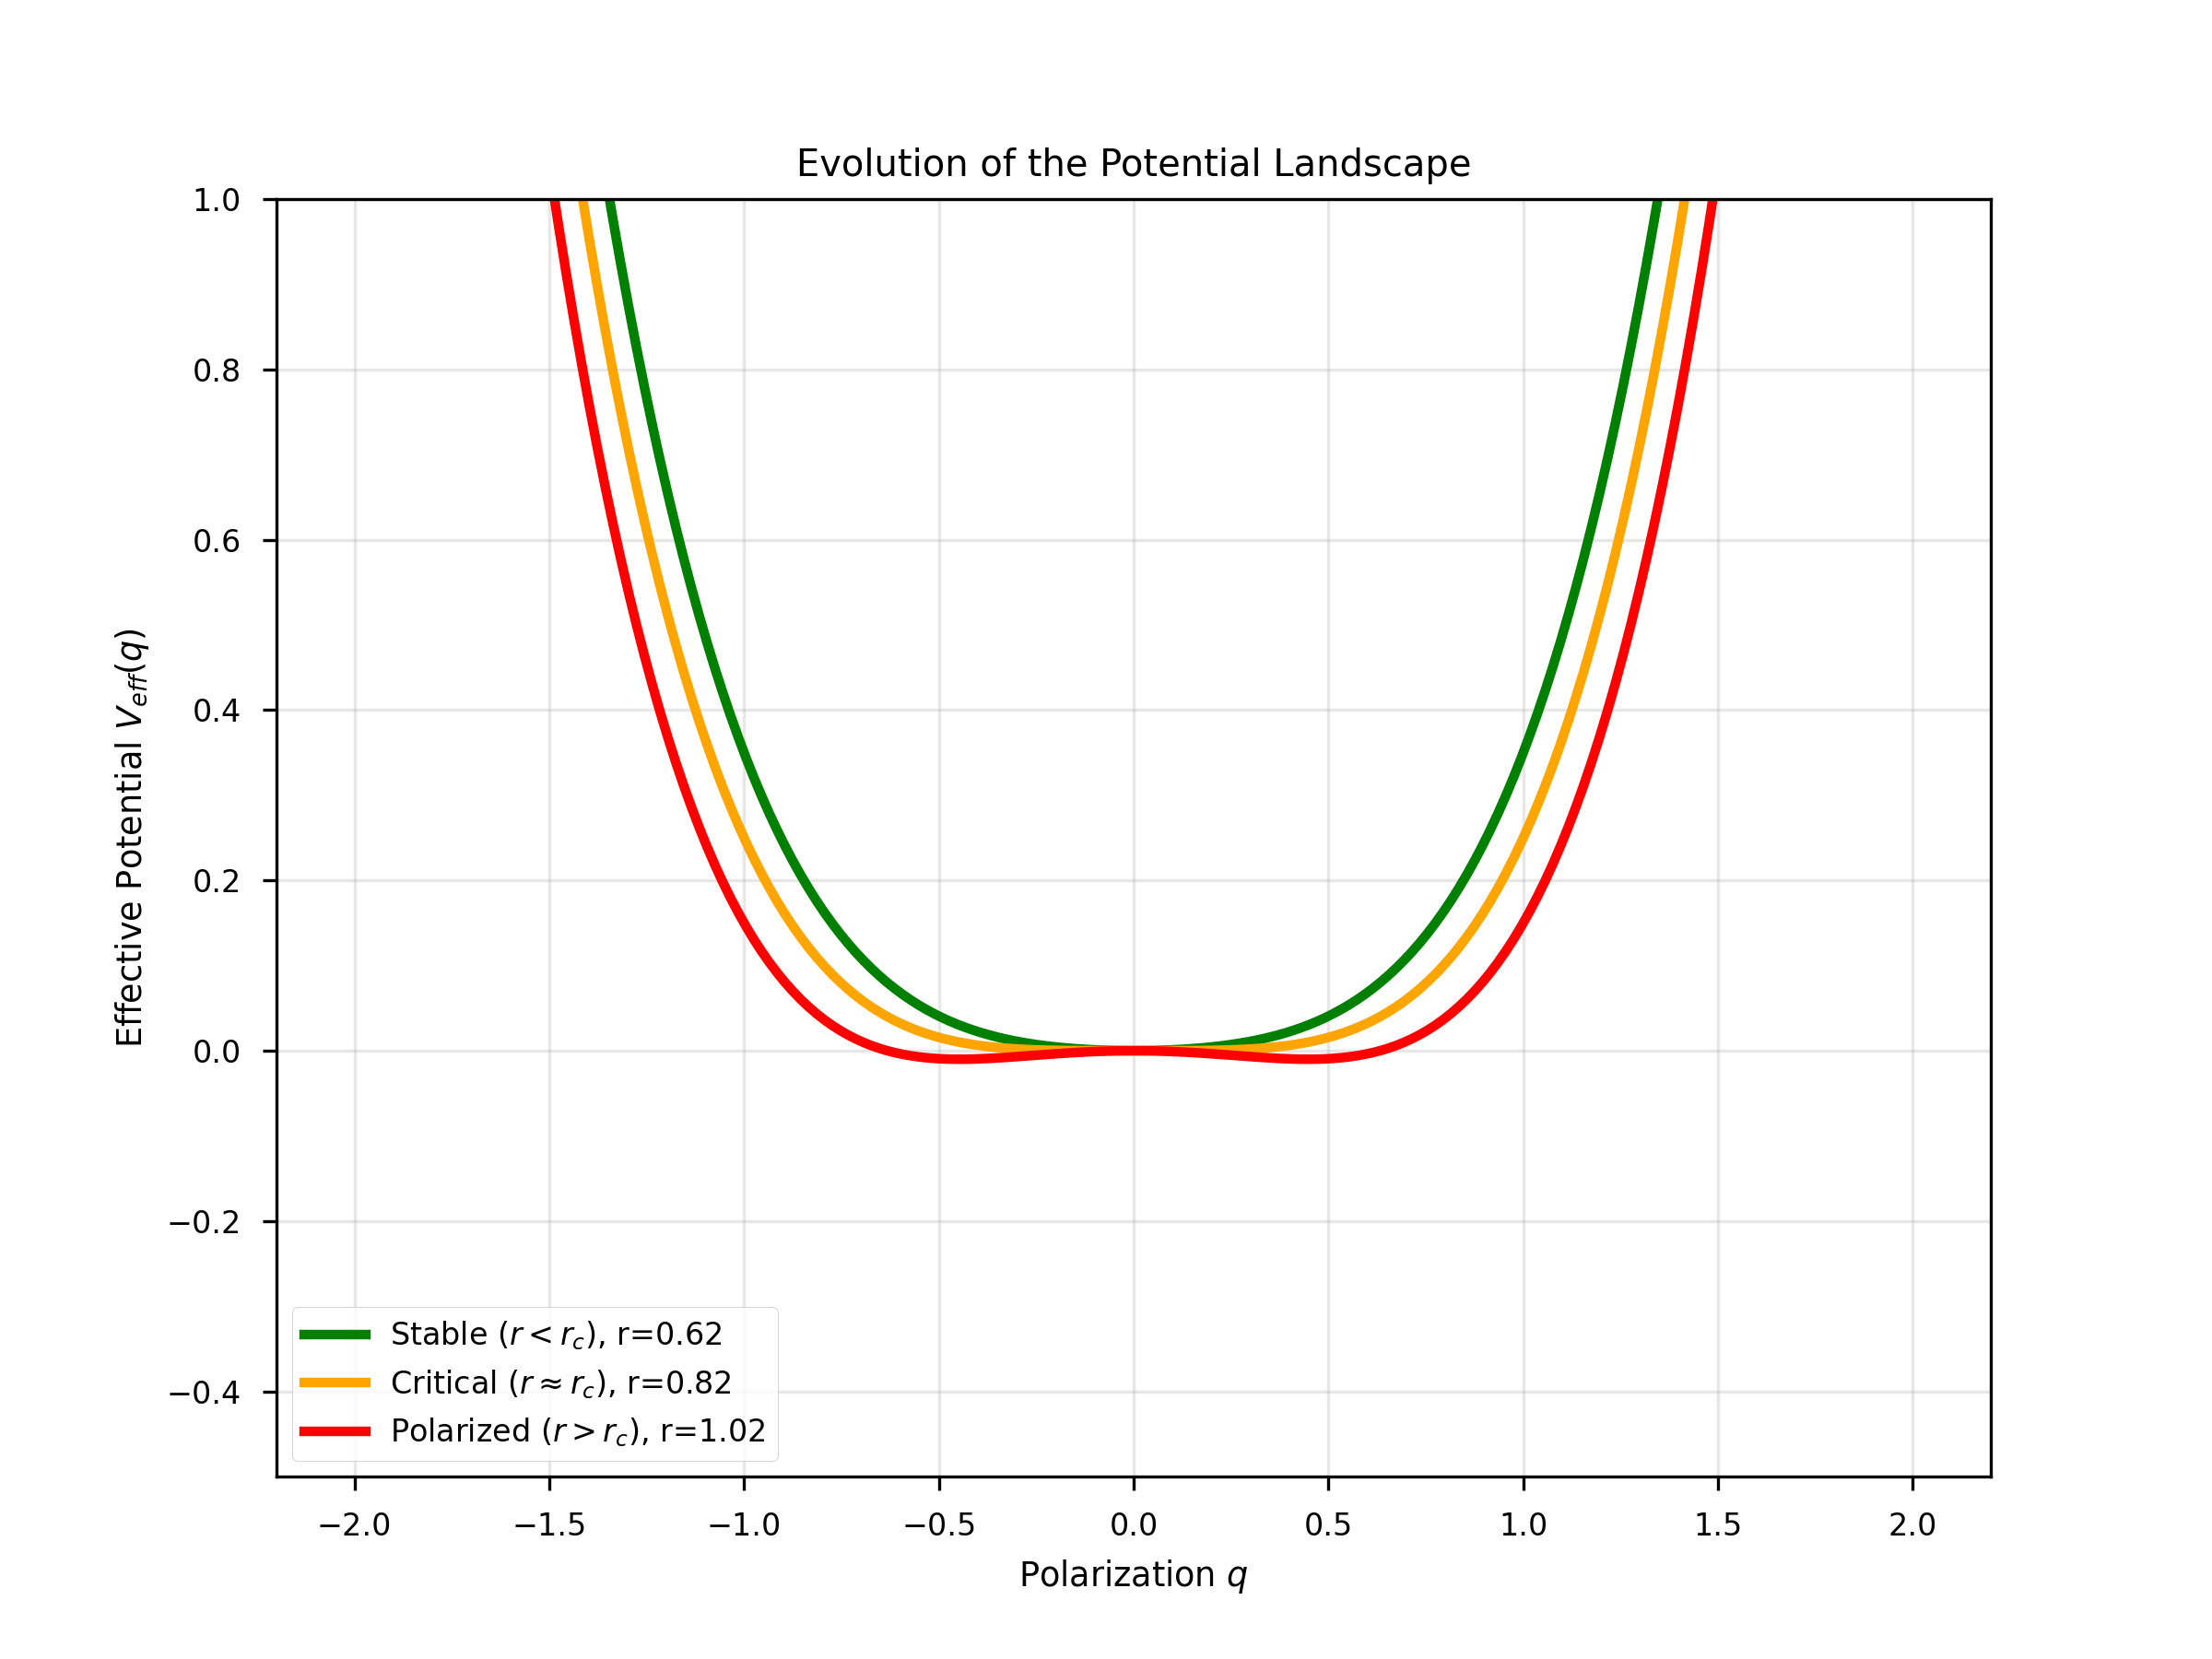
\includegraphics[width=\linewidth]{figures/fig1b_potential.png}
    \caption{}
  \end{subfigure}
  \caption{Theoretical bifurcation and effective potential in the symmetric regime. (a) The order parameter shows a pitchfork bifurcation near $r_c$. (b) The effective potential shifts from a single well to a double well as $r$ crosses $r_c$, explaining bistability and branch selection.}
  \label{fig:theory}
\end{figure}

\subsection{Network simulation validation and finite-size stability}
Agent-based simulations on ER and BA networks reproduce the mean-field bifurcation in the symmetric regime and clarify how measurement choices affect interpretation. Because branch selection is random in a symmetric system, the signed mean $\langle Q\rangle$ cancels; using $|Q|$ or aligned signed $Q$ recovers the expected bifurcation. Simulations also validate finite-size scaling using Binder cumulant crossings, which provide a more stable estimate of the transition than susceptibility peaks. Figure~\ref{fig:network} shows that the theoretical bifurcation persists under networked interactions, while finite-size diagnostics localize the critical region. In the asymmetric regime, the coupling between $(q,a)$ and local reinforcement can shift the effective transition point, indicating a structural mechanism rather than an implementation artifact.

\begin{figure}[t]
  \centering
  \begin{subfigure}[b]{0.48\linewidth}
    \centering
    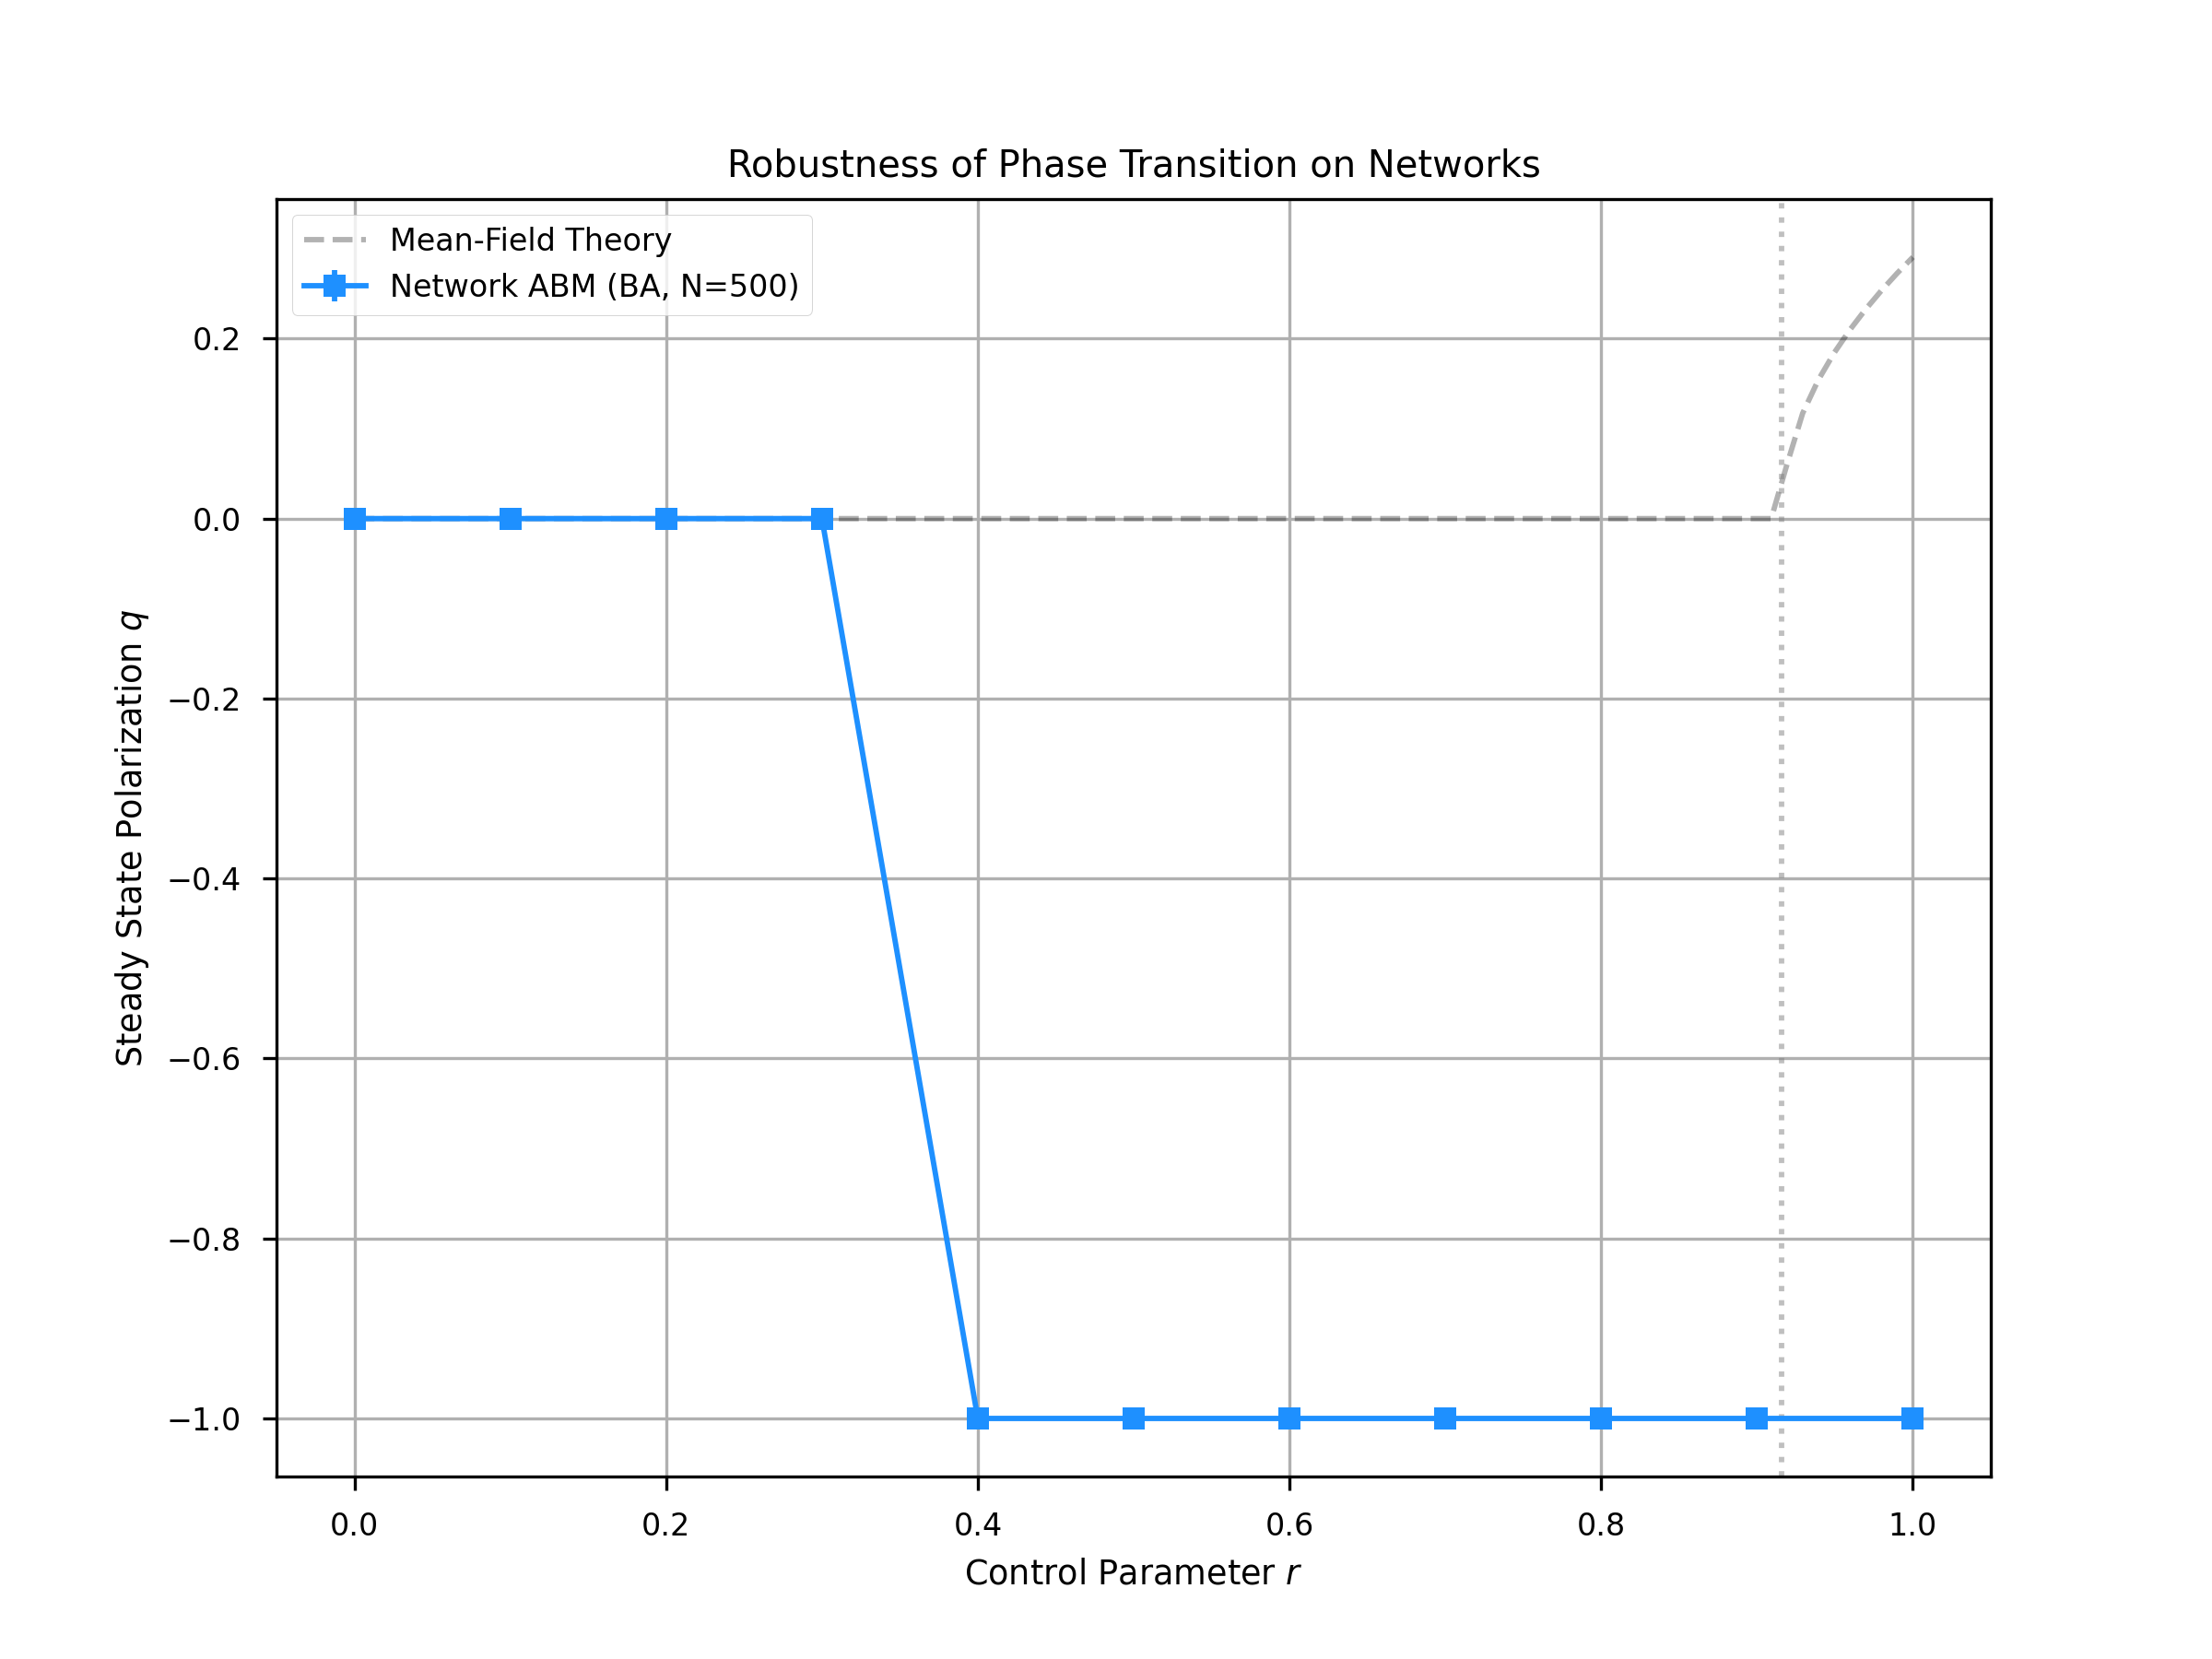
\includegraphics[width=\linewidth]{figures/fig2a_network_validation.png}
    \caption{}
  \end{subfigure}
  \hfill
  \begin{subfigure}[b]{0.48\linewidth}
    \centering
    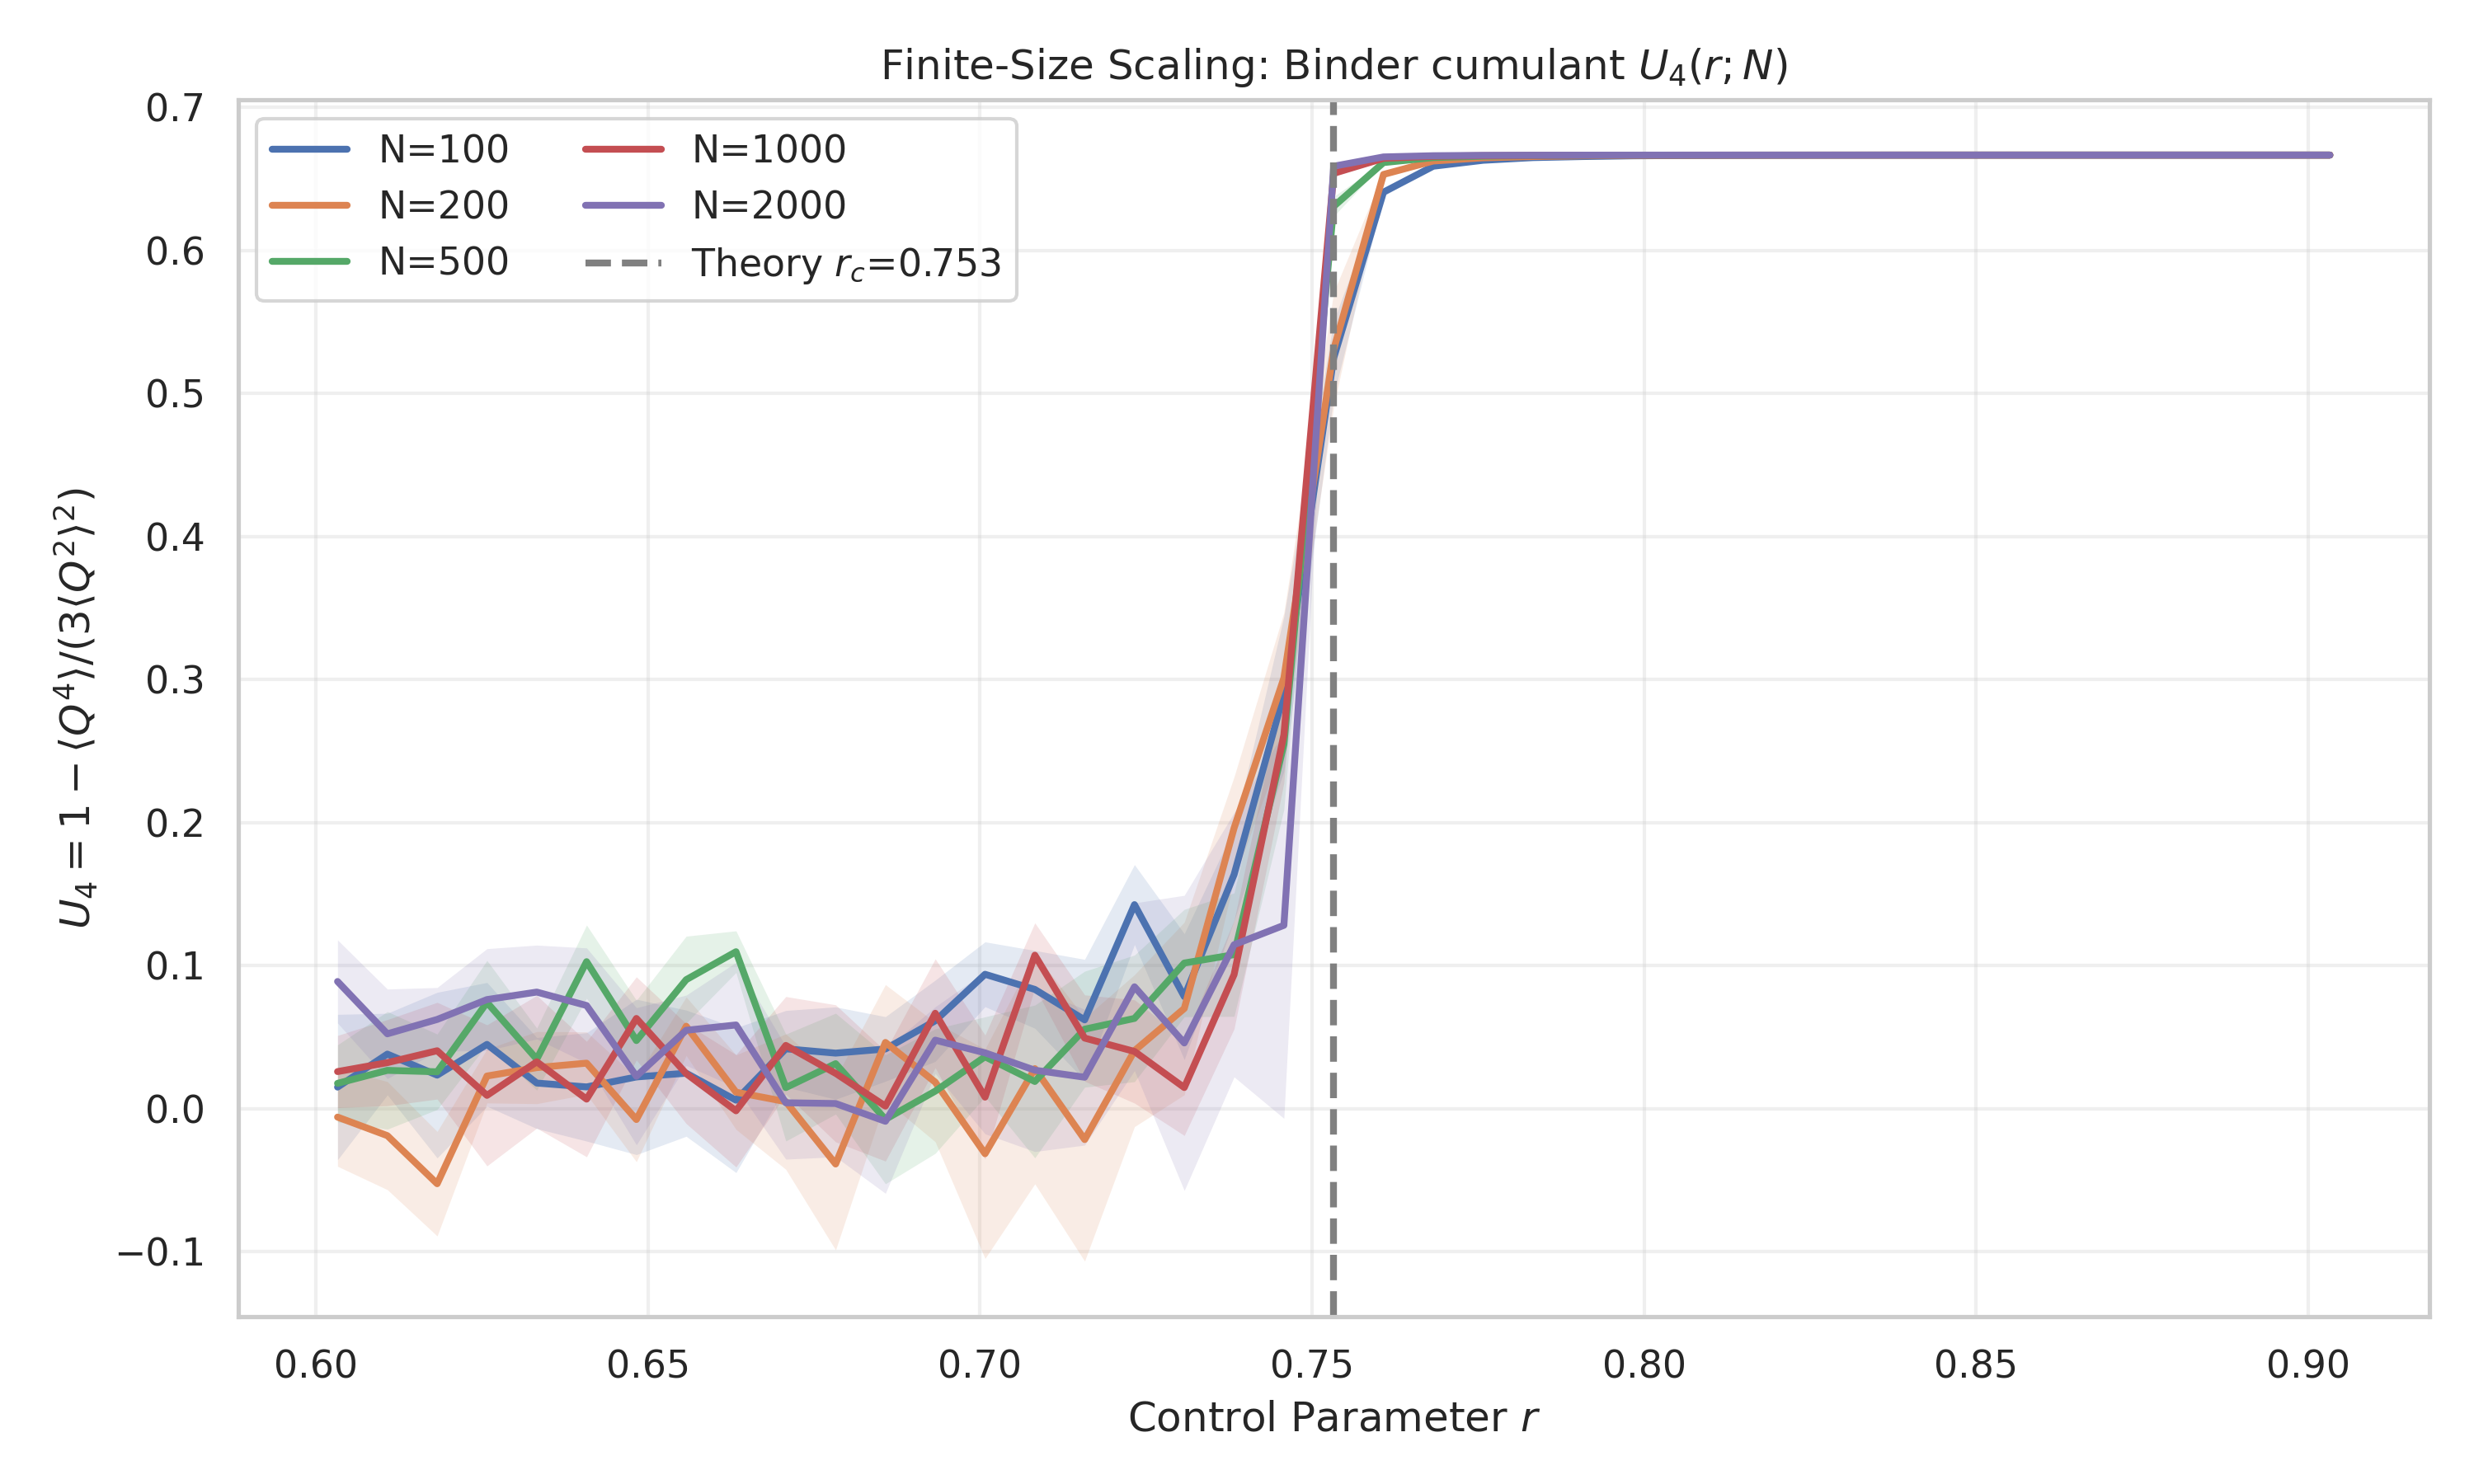
\includegraphics[width=\linewidth]{figures/fig2b_binder_u4.png}
    \caption{}
  \end{subfigure}
  \caption{Network validation and finite-size stability. (a) Agent-based simulations reproduce the theoretical bifurcation in the symmetric regime and reveal shifts under asymmetric coupling. (b) Binder cumulant $U_4(r;N)$ curves provide robust critical-region localization across system sizes.}
  \label{fig:network}
\end{figure}

\subsection{Critical slowing down and time-scale alignment}
Near $r_c$, the restoring force vanishes and the relaxation time diverges, yielding critical slowing down. We align the time scale between asynchronous ABM updates and continuous-time theory by converting steps to sweeps, and then evaluate autocorrelation and variance-based indicators. The simulations show increasing relaxation time and rising autocorrelation as $r$ approaches $r_c$, consistent with the theoretical prediction $\tau\sim 1/|r_c-r|$ (Fig.~\ref{fig:csd}). This alignment is essential for a consistent interpretation of early-warning signals across modeling layers.

\begin{figure}[t]
  \centering
  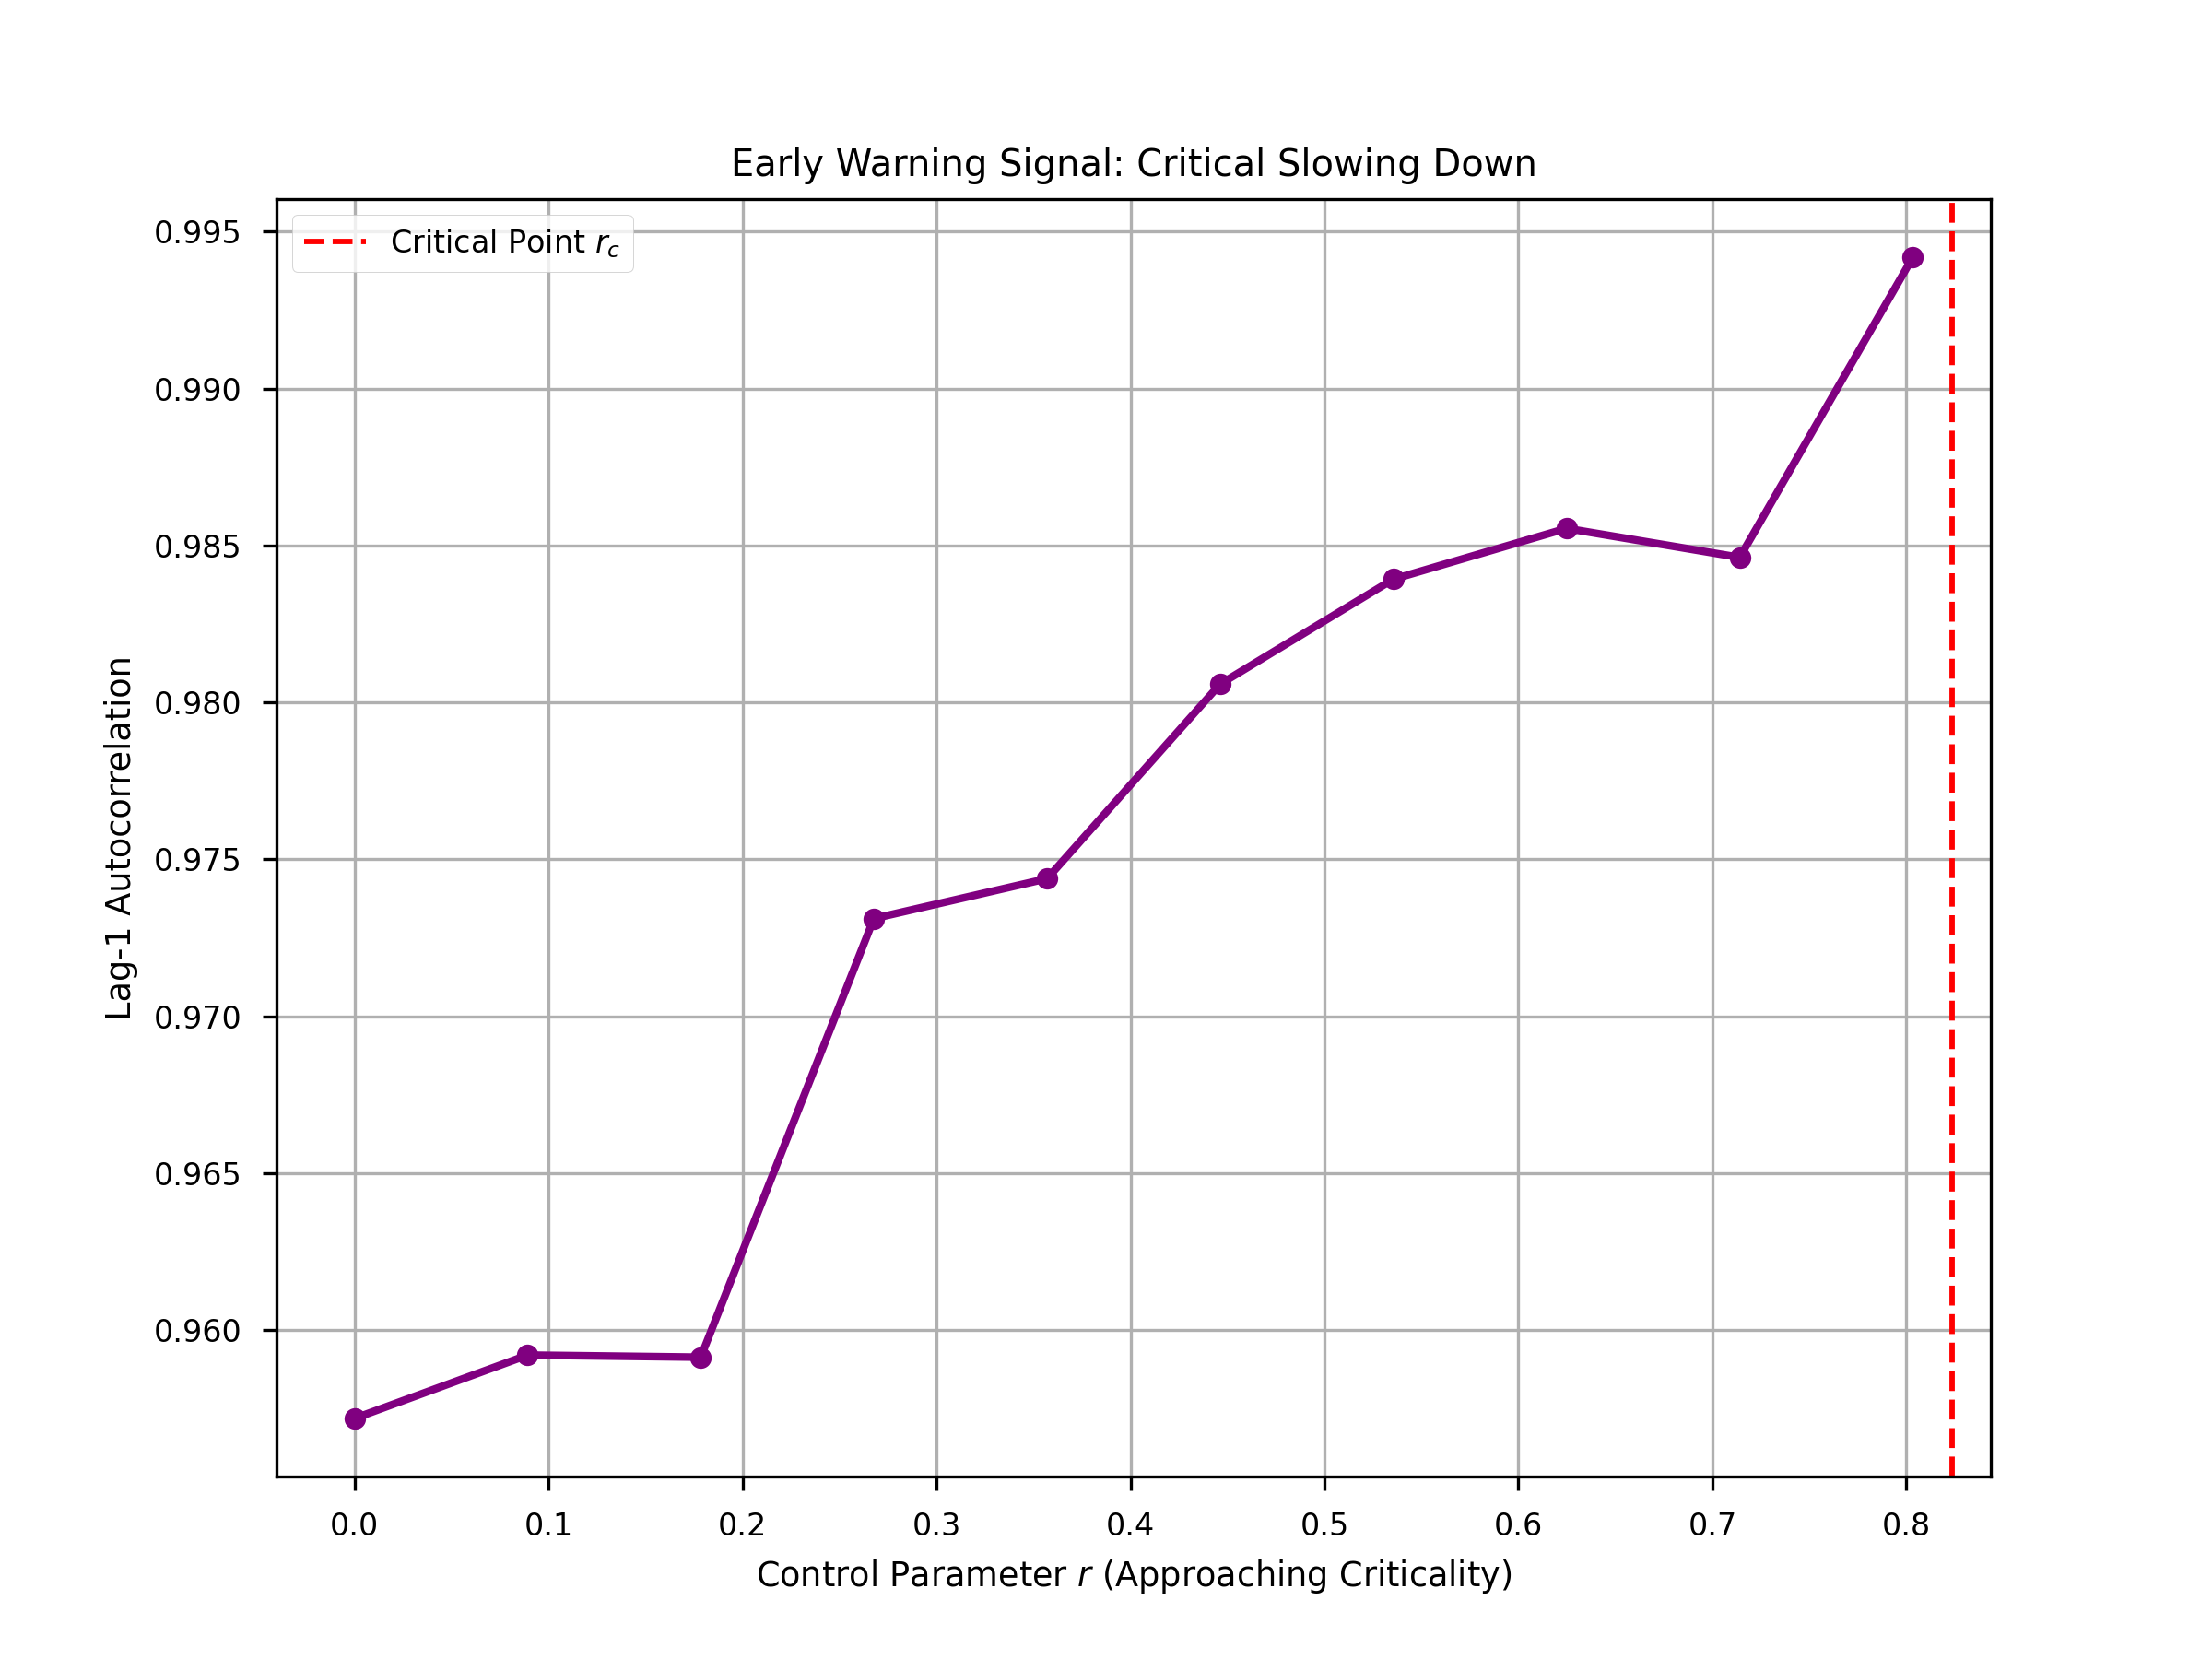
\includegraphics[width=0.9\linewidth]{figures/fig3_csd.png}
  \caption{Critical slowing down near the theoretical critical point. Relaxation time and autocorrelation-based indicators increase as $r\to r_c$, and the trend persists after aligning ABM steps with sweep-based time scales.}
  \label{fig:csd}
\end{figure}

\subsection{Parameter landscapes and structural effects}
The model predicts how psychological thresholds, information density, media ecology, and local coupling reshape the phase boundary. The sensitivity $\chi$ and the critical point $r_c$ vary systematically across $(\phi,\theta)$, and a transition exists only when $\chi>2$. Increasing information density $k$ generally raises $\chi$ and shifts $r_c$, while a higher We-media ratio lowers the effective transition point, indicating greater fragility. Local coupling $\beta$ re-parameterizes the macroscopic boundary by amplifying neighborhood reinforcement. These effects are consistent across mean-field calculations and network simulations (Fig.~\ref{fig:landscape}), showing that topology and media ecology jointly determine how close the system operates to criticality.

\begin{figure}[t]
  \centering
  \begin{subfigure}[b]{0.48\linewidth}
    \centering
    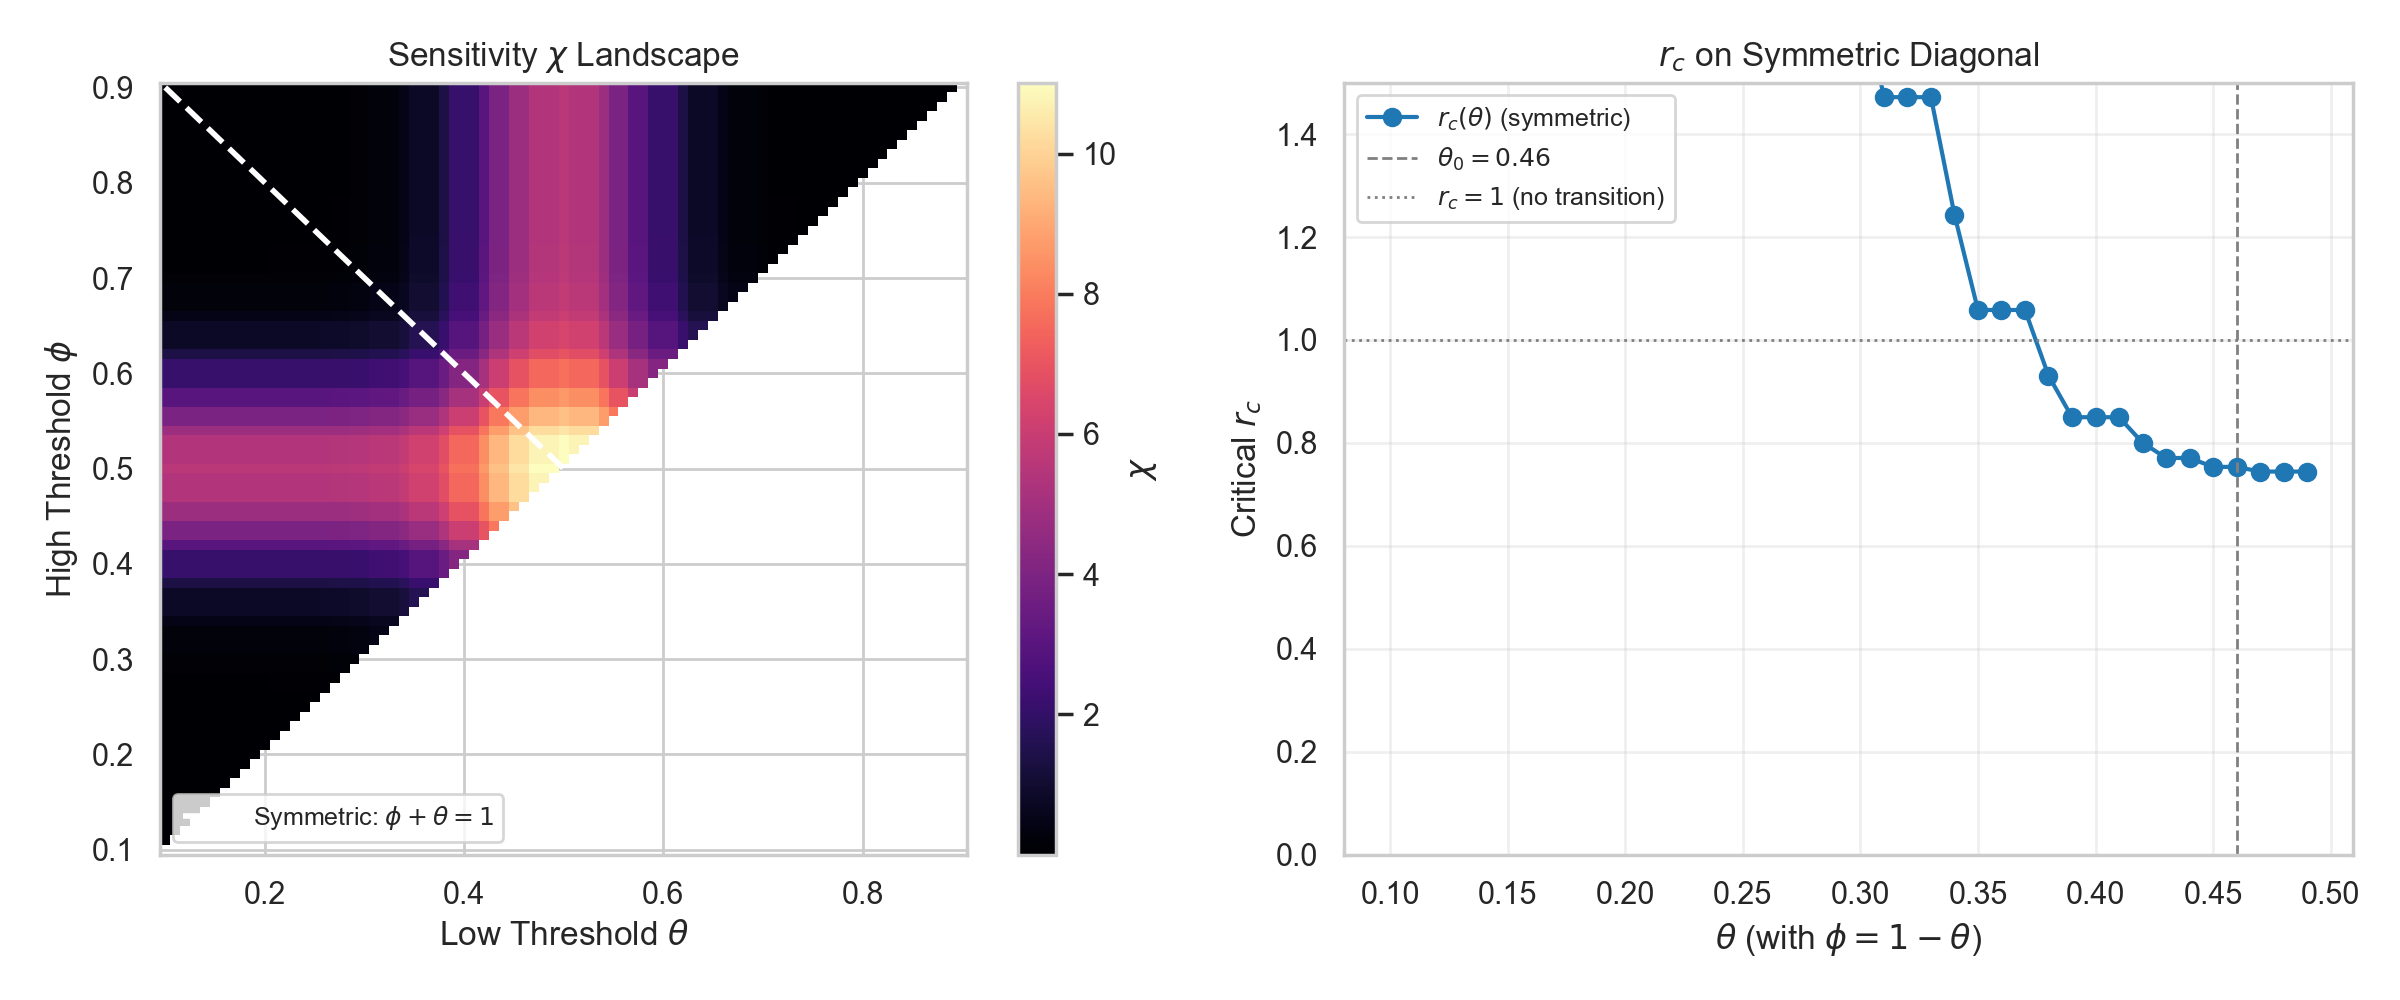
\includegraphics[width=\linewidth]{figures/fig4a_chi_rc_landscape.png}
    \caption{}
  \end{subfigure}
  \hfill
  \begin{subfigure}[b]{0.48\linewidth}
    \centering
    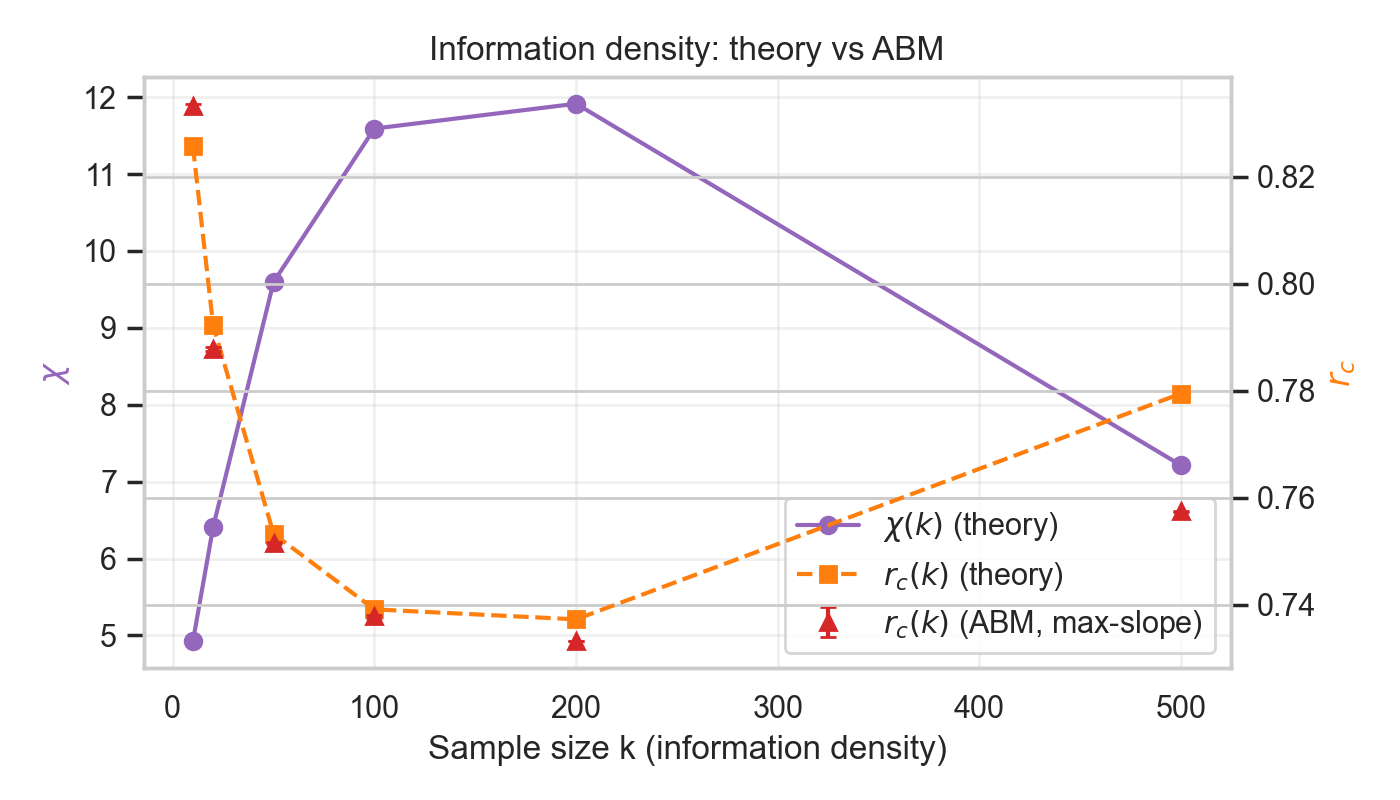
\includegraphics[width=\linewidth]{figures/fig4b_k_effect.png}
    \caption{}
  \end{subfigure}
  \vspace{0.5em}
  \begin{subfigure}[b]{0.48\linewidth}
    \centering
    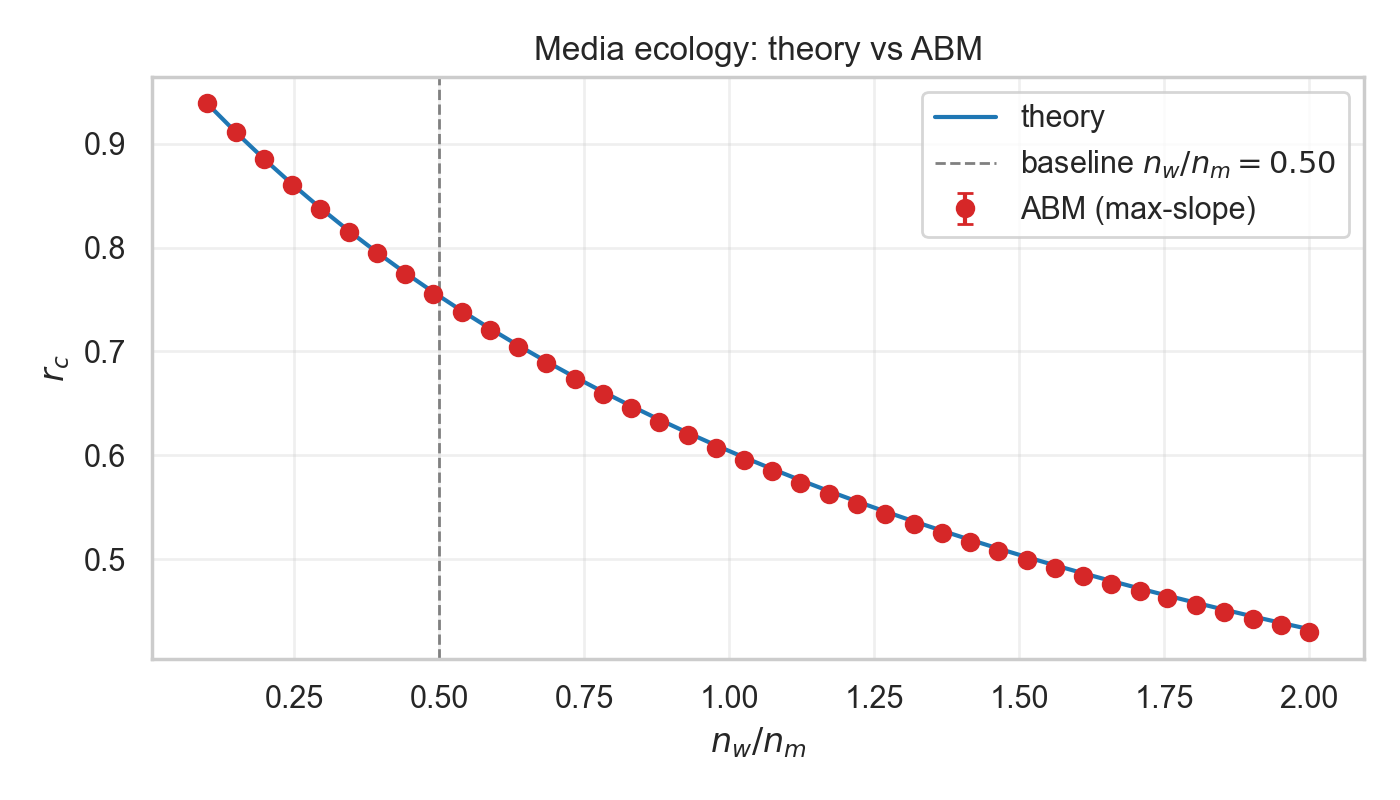
\includegraphics[width=\linewidth]{figures/fig4c_media_ratio.png}
    \caption{}
  \end{subfigure}
  \hfill
  \begin{subfigure}[b]{0.48\linewidth}
    \centering
    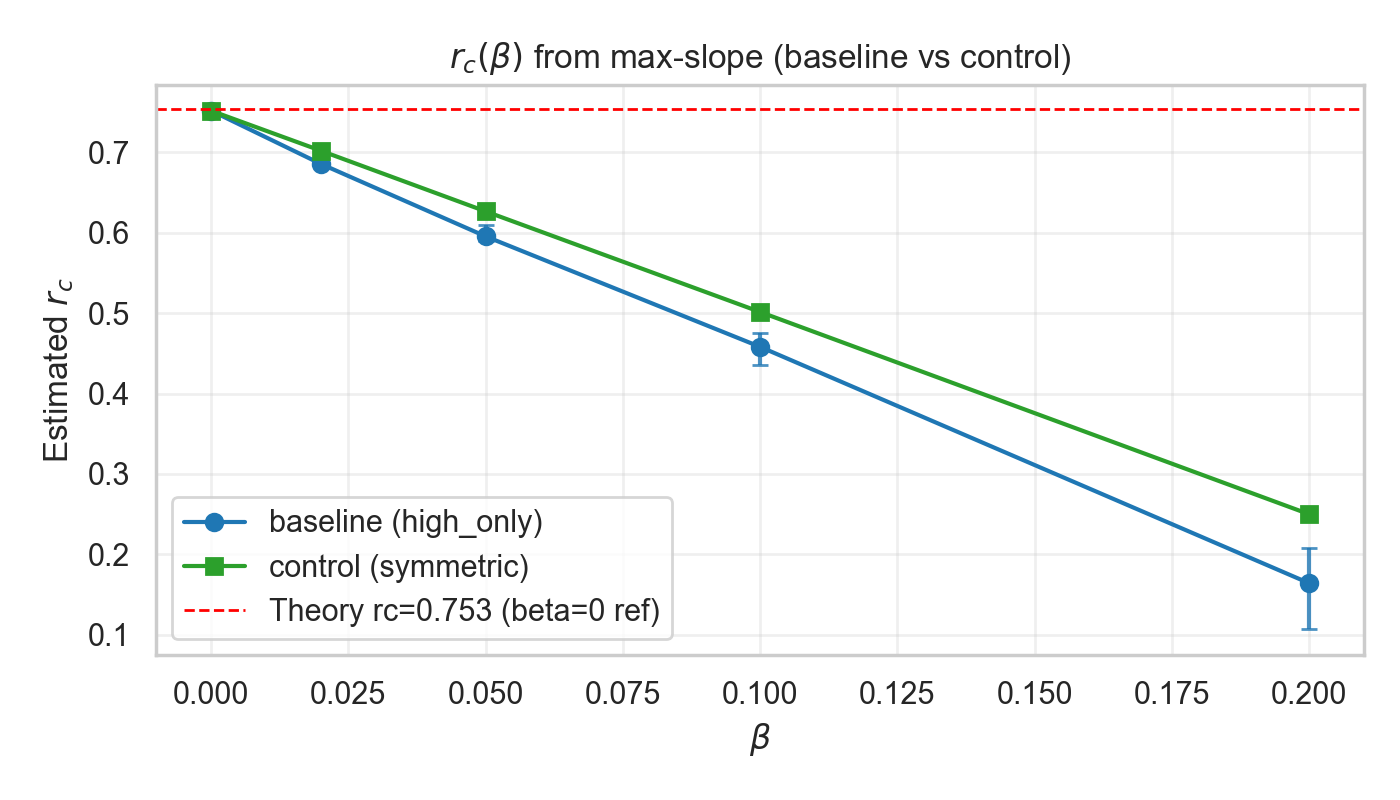
\includegraphics[width=\linewidth]{figures/fig4d_beta_effect.png}
    \caption{}
  \end{subfigure}
  \caption{Parameter landscapes and structural effects. (a) Sensitivity $\chi$ and $r_c$ across $(\phi,\theta)$. (b) Information density $k$ shifts $\chi$ and the effective transition. (c) Media ecology $n_w/n_m$ lowers $r_c$ as We-media dominance grows. (d) Local coupling $\beta$ re-parameterizes the effective transition boundary.}
  \label{fig:landscape}
\end{figure}

\subsection{Empirical validation of theoretical signatures}
We evaluate three empirical signatures on Weibo data using proxy mappings for $Q$, $a$, and $r_{\text{proxy}}$ under a pre-registered ``two-tier'' logic: (i) structure-level hypotheses are tested on datasets with larger cross-topic variance in $r_{\text{proxy}}$, and (ii) dynamical signatures are evaluated on cleaner within-topic time series. In the pooled dataset (master+batch3), the activity-to-jump hypothesis (H1) is supported: higher segment-level activity predicts larger jump intensity (Fig.~\ref{fig:empirical}a). For the media-volatility hypothesis (H2), batch3 shows a significant association between $r_{\text{proxy}}$ and volatility (Fig.~\ref{fig:empirical}b); however, this relationship weakens after controlling for segment-level sampling density, indicating an important confound. Finally, the critical slowing down signature (H4) is inconclusive: event-aligned $AC1(|Q|)$ and $\mathrm{Var}(|Q|)$ do not reliably exceed placebo baselines under the current data continuity and event counts (Fig.~\ref{fig:empirical}c), and higher temporal resolution (1H/2H) further breaks continuity, making H4 difficult to evaluate without denser time series.

\begin{table}[t]
  \centering
  \caption{Summary of empirical hypothesis tests under the primary 4H aggregation. Pearson correlations (p-values) are reported for H1 and H2. For H4, we report the number of detected events and one-sided block-aware placebo p-values for $AC1(|Q|)$ and $\mathrm{Var}(|Q|)$. In batch3, the H2 association weakens after controlling for segment-level sampling density (partial $r=0.078$, $p=0.411$), indicating a confound.}
  \label{tab:empirical}
  \begin{tabular}{lccc}
    \hline
    Hypothesis & Batch1 (single topic) & Batch3 & All (master+batch3) \\
    \hline
    H1: Activity $\to$ Jump & $r=-0.349$ ($p=0.293$) & $r=0.159$ ($p=0.090$) & $r=0.241$ ($p=0.00798$) \\
    H2: $r_{\text{proxy}}\to$ Volatility & $r=0.098$ ($p=0.774$) & $r=0.265$ ($p=0.00434$) & $r=0.065$ ($p=0.484$) \\
    H4: CSD before jumps & events=2; $p_{AC1}=0.525$; $p_{\mathrm{Var}}=0.537$ & events=13; $p_{AC1}=0.571$; $p_{\mathrm{Var}}=0.905$ & events=16; $p_{AC1}=0.359$; $p_{\mathrm{Var}}=0.843$ \\
    \hline
  \end{tabular}
\end{table}

\begin{figure}[t]
  \centering
  \begin{subfigure}[b]{0.48\linewidth}
    \centering
    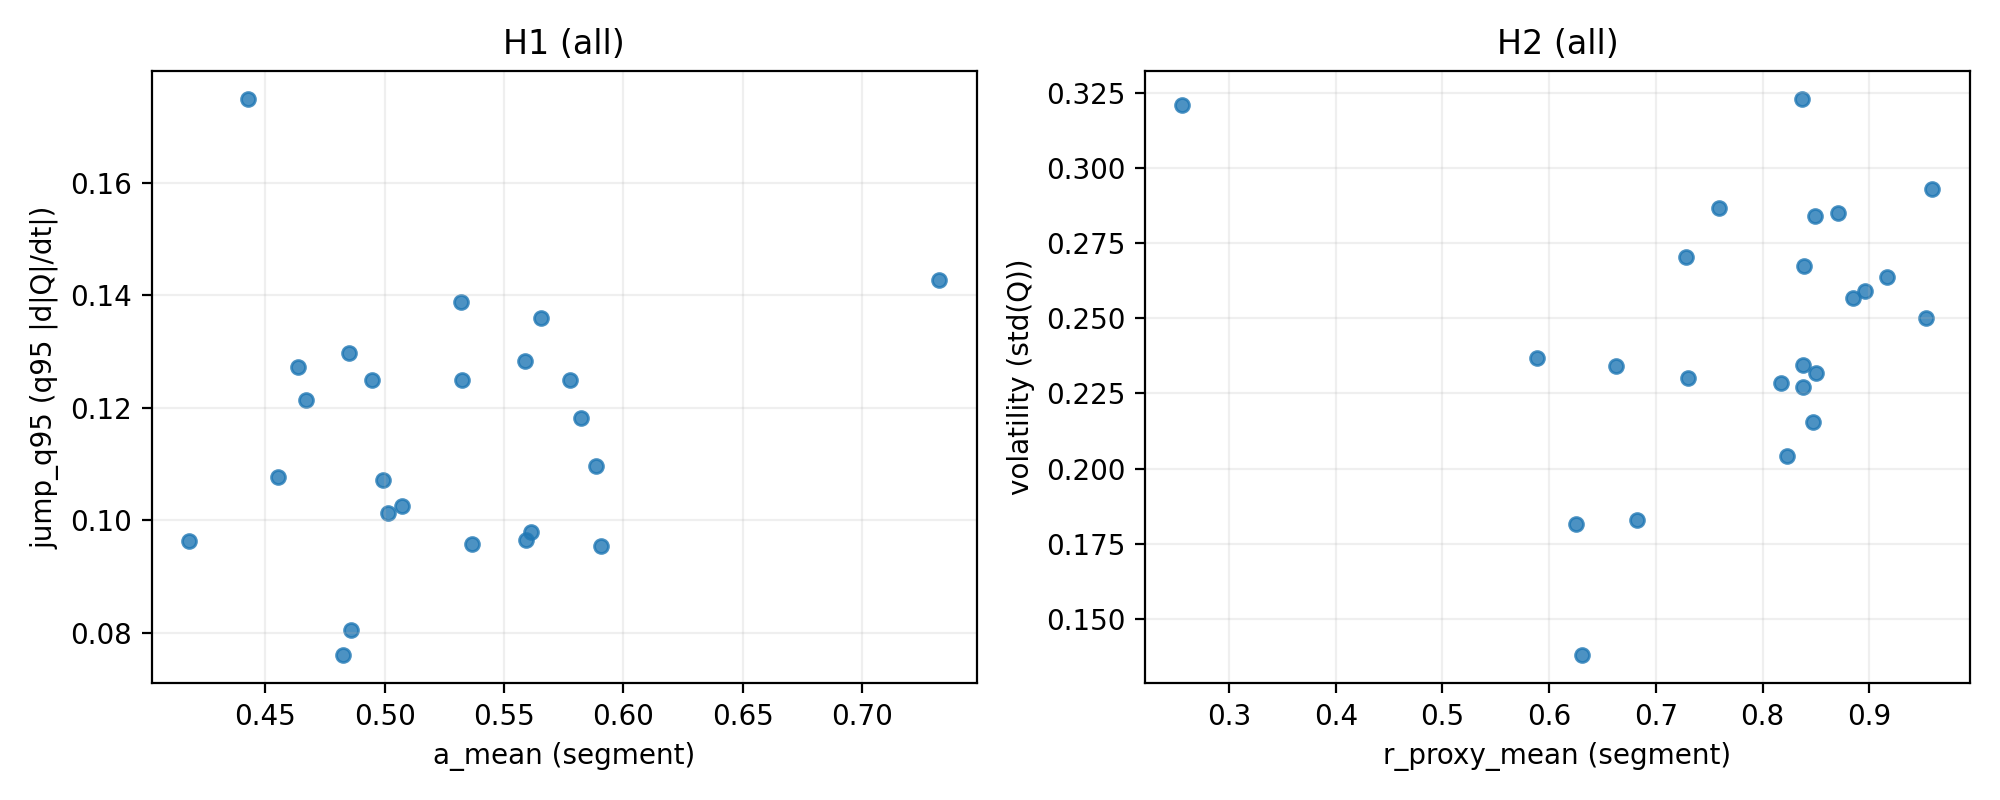
\includegraphics[width=\linewidth]{figures/fig5a_h1_all.png}
    \caption{}
  \end{subfigure}
  \hfill
  \begin{subfigure}[b]{0.48\linewidth}
    \centering
    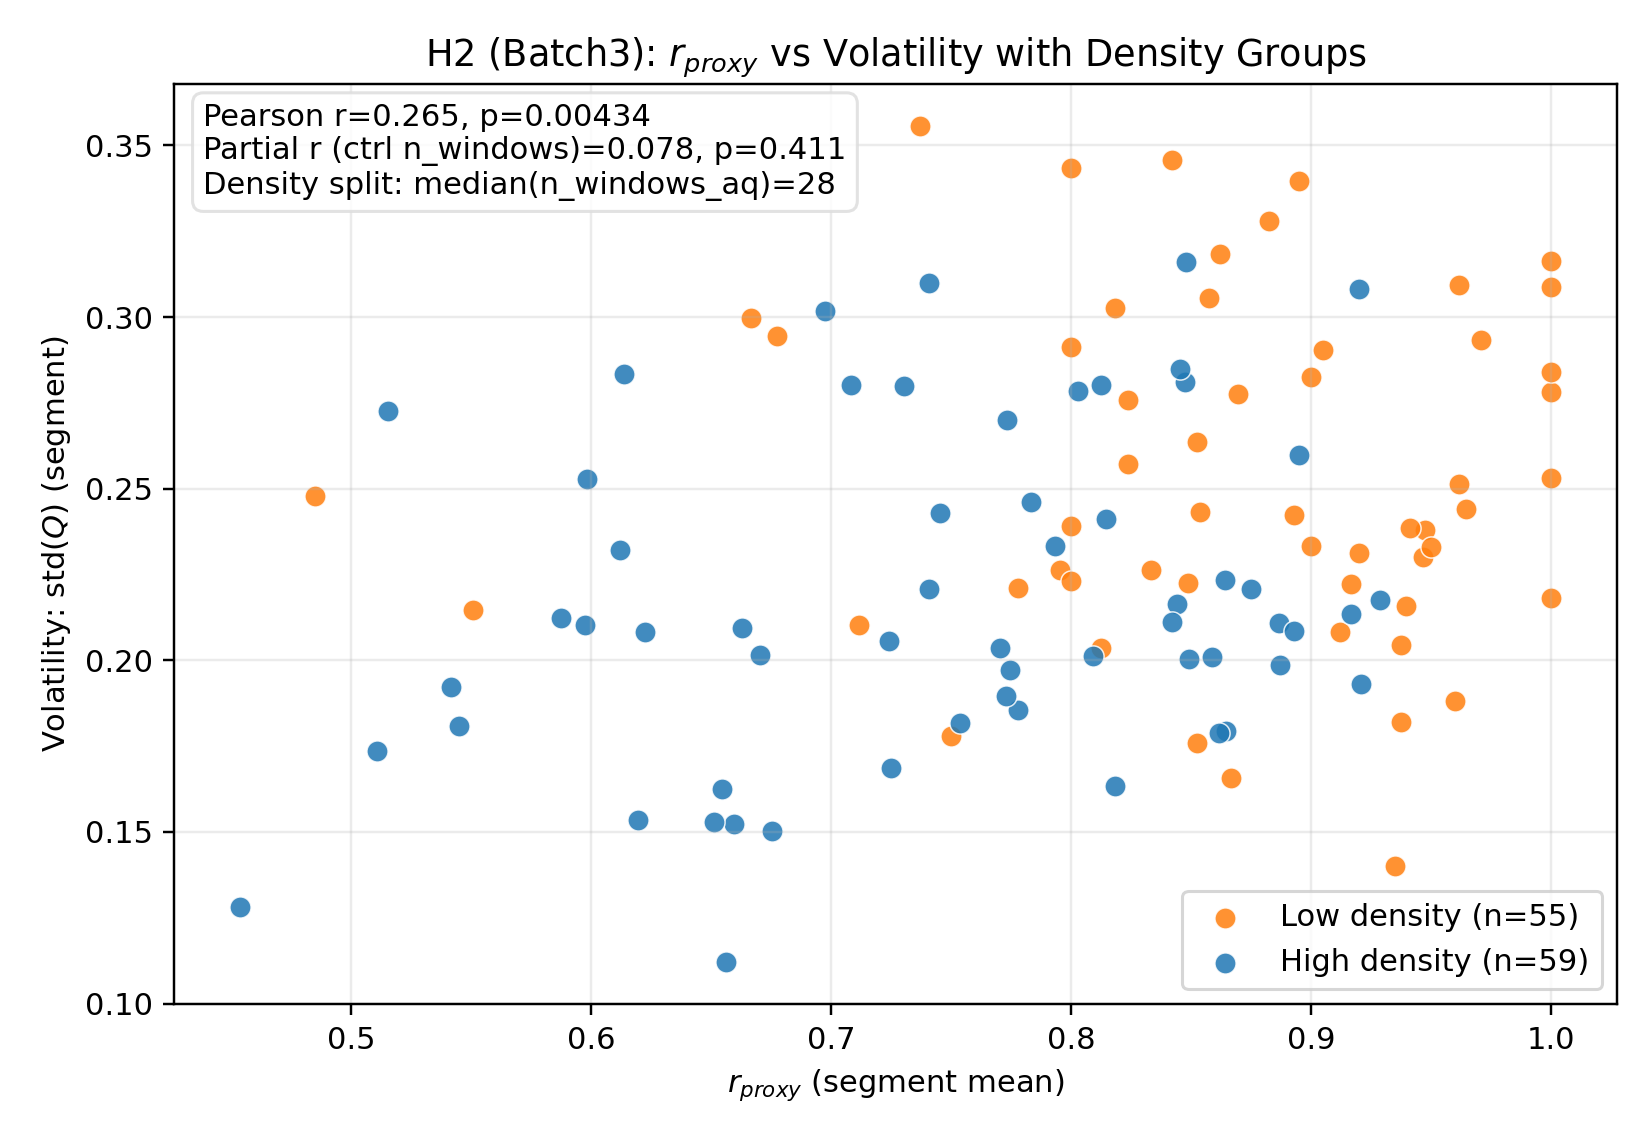
\includegraphics[width=\linewidth]{figures/fig5b_h2_batch3_density.png}
    \caption{}
  \end{subfigure}
  \vspace{0.6em}
  \begin{subfigure}[b]{0.7\linewidth}
    \centering
    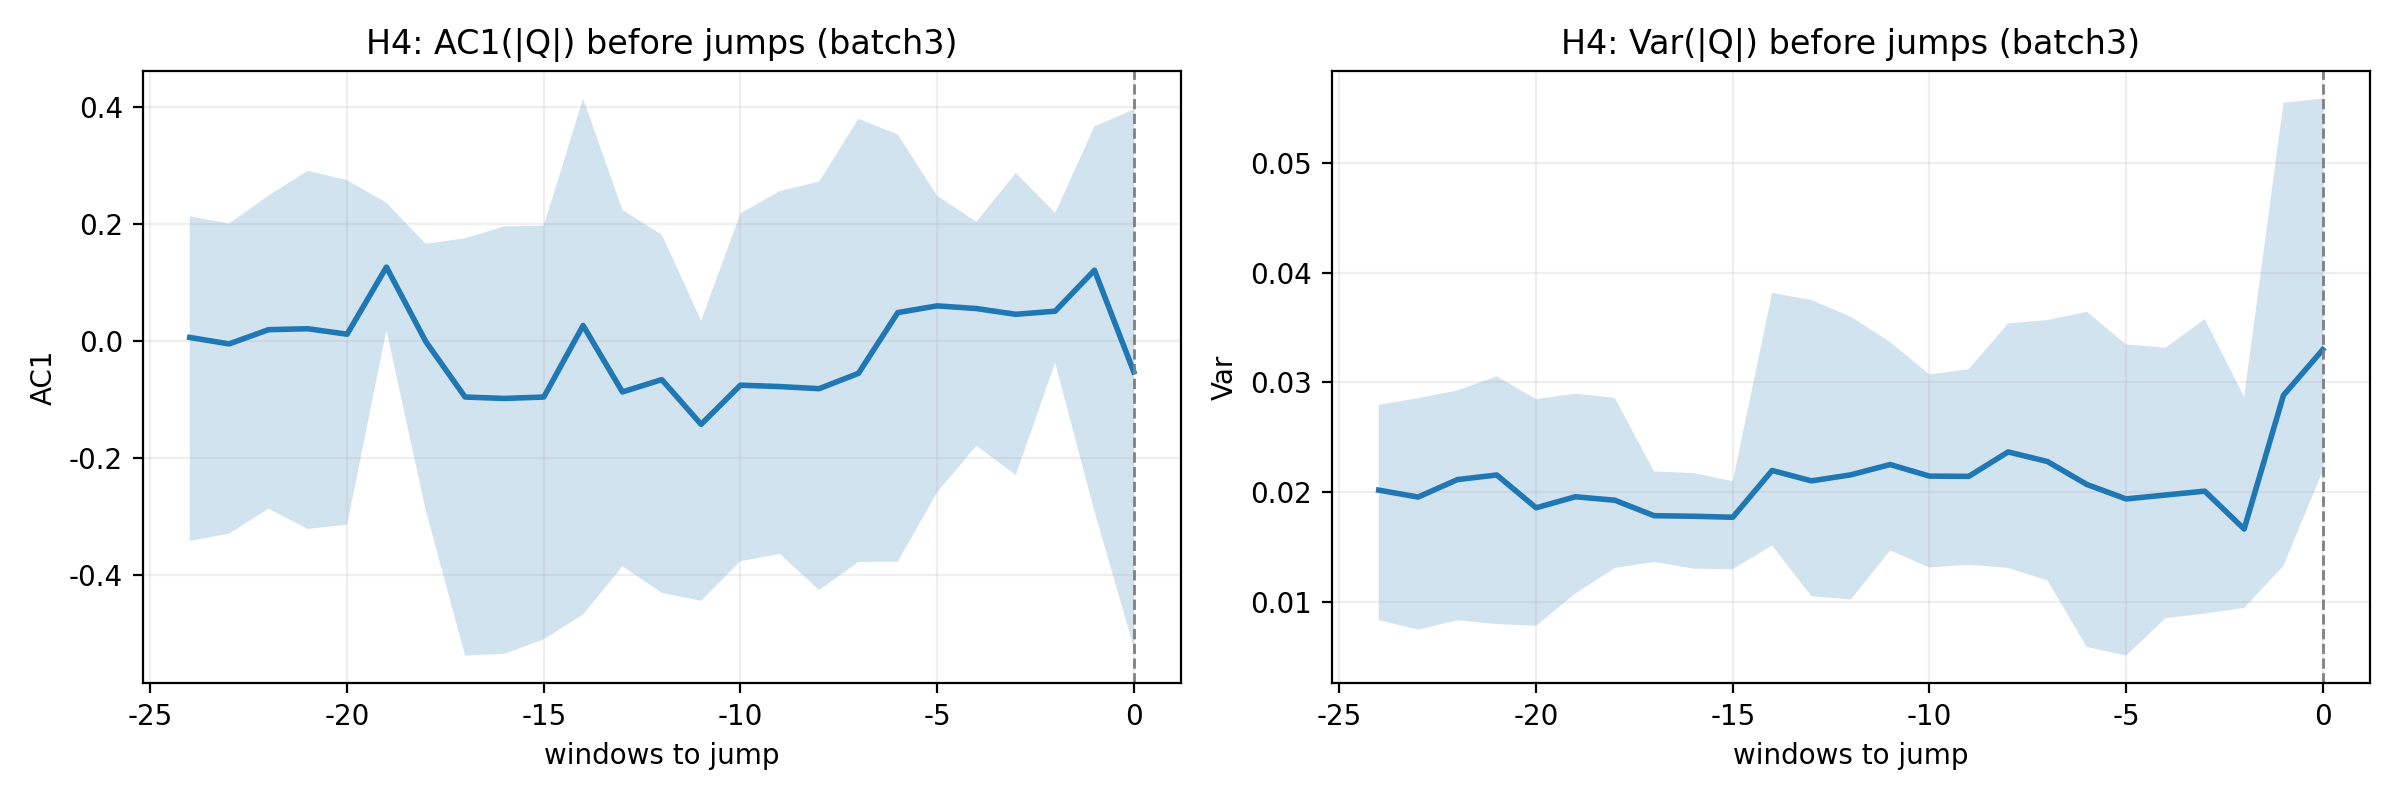
\includegraphics[width=\linewidth]{figures/fig5c_h4_event_batch3.png}
    \caption{}
  \end{subfigure}
  \caption{Empirical validation of theoretical signatures. (a) H1: segment-level activity $a$ versus jump intensity ($\text{jump}_{q95}$ of $|d|Q|/dt|$) in the pooled dataset, showing a significant positive association. (b) H2: $r_{\text{proxy}}$ versus volatility in batch3; the raw association is significant, while density controls weaken the effect, indicating a confound. (c) H4: event-aligned $AC1(|Q|)$ and $\mathrm{Var}(|Q|)$ show limited evidence for critical slowing down and do not robustly exceed placebo baselines under current sampling density and continuity.}
  \label{fig:empirical}
\end{figure}

\section{Discussion}
This study develops a mixed-feedback theory of collective emotion that links competing media dynamics to phase-transition behavior. The model provides an analytic critical point, a Ginzburg-Landau interpretation of bistability, and predictions about slowing dynamics near criticality. These predictions are supported by agent-based simulations and finite-size diagnostics, while parameter landscapes clarify how psychological thresholds, information density, media ecology, and local coupling shift fragility.

Empirical validation provides partial support under the PI-adopted two-tier strategy. H1 is supported in the pooled dataset: higher activity predicts larger jump intensity, consistent with the idea that depleted moderation buffers increase fragility. H2 is supported in batch3, where $r_{\text{proxy}}$ is significantly associated with volatility, but the effect weakens under density controls, indicating that sampling density is a key confound that should be reported transparently. Evidence for critical slowing down (H4) is inconclusive: event-aligned $AC1(|Q|)$ and $\mathrm{Var}(|Q|)$ do not robustly exceed placebo baselines, and attempts to increase temporal resolution (1H/2H) can make H4 non-evaluable due to broken continuity. This negative result is informative: it delineates a practical boundary for detecting early-warning signals in noisy, sparse social media time series.

Several limitations point to future extensions. The model treats media sources as homogeneous within each class; weighting by credibility, audience size, or engagement could yield more realistic feedback. The population is homogeneous, whereas psychological thresholds likely vary by demographic group \citep{Schwartz2013,Pfefferbaum2020}. Network structure can also be richer than ER or BA graphs, with homophily and community structure shaping diffusion \citep{Bisgin2012,Dandekar2013,McPherson2001}. On the empirical side, denser and more continuous time series are needed to test critical slowing down with sufficient power; otherwise, higher-frequency aggregation can reduce evaluability rather than improve it. Addressing these limitations would strengthen causal inference about media-driven sentiment fragility and clarify when early-warning monitoring is feasible in practice.

\section*{Appendix: Sensitivity to Time Aggregation and Data Continuity}
To reduce potential over-smoothing at 4H aggregation, we tested 2H and 1H resolutions while keeping comparable window durations (e.g., $\sim$48h rolling and $\sim$96h pre-event lookback). In practice, finer aggregation amplifies missingness and shortens continuous blocks, which breaks the rolling-window assumptions needed for $AC1(|Q|)$ and $\mathrm{Var}(|Q|)$. Under strict block-aware evaluation, this can yield zero eligible windows and thus zero detectable events (eligible=0/events=0), making H4 non-evaluable. This sensitivity indicates that, despite a clear theoretical prediction, empirical detection of critical slowing down in social media data requires substantially denser and more continuous sampling.

\FloatBarrier
\bibliographystyle{unsrt}
\bibliography{references}

\end{document}
